\documentclass[reqno]{amsart}

\usepackage{enumerate, amsmath, amsfonts, amssymb, amsthm, wasysym, graphics, graphicx, xcolor, url, hyperref, hypcap, a4wide, pdflscape, multido, xargs, colortbl, multicol, multirow, calc, shuffle}
\hypersetup{colorlinks=true, citecolor=PineGreen, linkcolor=PineGreen}
%\usepackage[all]{xy}
\usepackage{tikz}\usetikzlibrary{trees,snakes,shapes,arrows,matrix,calc}
\usepackage{comment}
\usepackage{etex}
\usepackage{ulem}\normalem % to strike through a word
\usepackage[noabbrev,capitalise]{cleveref}

%\reserveinserts{50}
\graphicspath{{figures/}}
\makeatletter
\def\input@path{{figures/}}
\makeatother

%%%%%%%%%%%%%%%%%%%%%%%%%%%%%%%%%%%%%%

\title{Lattices of acyclic pipe dreams}

\author[N.~Bergeron]{Nantel Bergeron} 
\address[N.~Bergeron]{Department of Mathematics and Statistics, York University, Toronto}
\email{bergeron@yorku.ca}
\urladdr{http://bergeron.mathstats.yorku.ca}

\author[N.~Cartier]{No\'emie Cartier} 
\address[N.~Cartier]{LRI, Université Paris Saclay}
\email{noemie.cartier@lri.fr}

\author[C.~Ceballos]{Cesar Ceballos}
\address[C.~Ceballos]{Institute of Geometry, Technische Universit\"at Graz}
\email{cesar.ceballos@tugraz.at}
\urladdr{http://www.geometrie.tugraz.at/ceballos/}

\author[V.~Pilaud]{Vincent Pilaud}
\address[V.~Pilaud]{CNRS \& LIX, \'Ecole Polytechnique, Palaiseau}
\email{vincent.pilaud@lix.polytechnique.fr}
\urladdr{http://www.lix.polytechnique.fr/~pilaud/}

\thanks{NC \& VP were partially supported by the French project CHARMS (ANR~19\,CE40\,0017), and by the French\,--\,Austrian project PAGCAP (ANR~21\,CE48\,0020 \& FWF I 5788).}

%%%%%%%%%%%%%%%%%%%%%%%%%%%%%%%%%%%%%%

% theorems
\newtheorem{theorem}{Theorem}[section]
\newtheorem{theoremA}{Theorem}
\renewcommand{\thetheoremA}{\Alph{theoremA}}
\newtheorem{corollary}[theorem]{Corollary}
\newtheorem{proposition}[theorem]{Proposition}
\newtheorem{lemma}[theorem]{Lemma}
\newtheorem{conjecture}[theorem]{Conjecture}
\crefname{conjecture}{Conjecture}{Conjectures}
\newtheorem{conjectureA}{Conjecture}
\renewcommand{\theconjectureA}{\Alph{conjectureA}}
\crefname{conjectureA}{Conjecture}{Conjectures}

\theoremstyle{definition}
\newtheorem{definition}[theorem]{Definition}
\newtheorem{example}[theorem]{Example}
\newtheorem{remark}[theorem]{Remark}
\newtheorem{question}[theorem]{Question}
\newtheorem{notation}[theorem]{Notation}

% newcommands
% math special letters
\newcommand{\R}{\mathbb{R}} % reals
\newcommand{\N}{\mathbb{N}} % naturals
\newcommand{\Z}{\mathbb{Z}} % integers
\newcommand{\I}{\mathbb{I}} % set of integers
\newcommand{\C}{\mathbb{C}} % set of summands
\renewcommand{\b}[1]{\boldsymbol{#1}} % bold

% math commands
\newcommand{\set}[2]{\left\{ #1 \;\middle|\; #2 \right\}} % set notation
\newcommand{\bigset}[2]{\big\{ #1 \;|\; #2 \big\}} % big set notation
\newcommand{\biggset}[2]{\bigg\{ #1 \;\bigg|\; #2 \bigg\}} % big set notation
\newcommand{\multiset}[2]{\left\{\!\!\left\{ #1 \;\middle|\; #2 \right\}\!\!\right\}} % multiset notation
\newcommand{\bigmultiset}[2]{\big\{\!\!\big\{ #1 \;|\; #2 \big\}\!\!\big\}} % big multiset notation
\newcommand{\ssm}{\smallsetminus} % small set minus
\newcommand{\dotprod}[2]{\langle #1 | #2 \rangle} % dot product
\newcommand{\symdif}{\triangle} % symmetric difference
\newcommand{\one}{{1\!\!1}} % the all one vector
\newcommand{\eqdef}{\mbox{\,\raisebox{0.2ex}{\scriptsize\ensuremath{\mathrm:}}\ensuremath{=}\,}} % :=
\newcommand{\defeq}{\mbox{~\ensuremath{=}\raisebox{0.2ex}{\scriptsize\ensuremath{\mathrm:}} }} % =:
\newcommand{\polar}{^\diamond} % polar
\newcommand{\simplex}{\triangle} % simplex

% operators
\DeclareMathOperator{\conv}{conv} % convex hull
\DeclareMathOperator{\cone}{cone} % cone hull
\DeclareMathOperator{\arr}{Arr} % arrangements
\DeclareMathOperator{\Inv}{Inv} % inversion set
\DeclareMathOperator{\Ninv}{Ninv} % non-inversion set
\DeclareMathOperator{\DemazureProduct}{Dem} % non-inversion set

% others
\newcommand{\fix}[1]{{\bf FIXME: }#1} % emphasis of a problem to FIX
\newcommand{\ie}{\textit{i.e.}~} % id est
\newcommand{\eg}{\textit{e.g.}~} % exempli gratia
\newcommand{\Eg}{\textit{E.g.}~} % exempli gratia
\newcommand{\aka}{\textit{aka.}~} % also known as
\newcommand{\viceversa}{\textit{vice versa}} % vice versa
\newcommand{\ordinal}{\textsuperscript{th}} % th for ordinals
\newcommand{\ex}[1]{^{\textrm{ex#1}}} % example
\newcommand{\para}[1]{\medskip\noindent\textbf{#1}} % paragraph
\newcommand{\subpara}[1]{\smallskip\noindent\textit{#1.}} % paragraph
\definecolor{PineGreen}{RGB}{2,120,120} % pinegreen color
\definecolor{darkgreen}{RGB}{57,181,74} % darkgreen color
\newcommand{\blue}[1]{{\color{blue} #1}} % blue
\newcommand{\red}[1]{{\color{red} #1}} % red
\newcommand{\green}[1]{{\color{darkgreen} #1}} % green
\newcommand{\defn}[1]{\textbf{\textsf{\color{PineGreen} #1}}} % emphasis of a definition
\usepackage{todonotes}
\newcommand{\nantel}[1]{\todo[color=red!30]{#1 \\ \hfill --- N.}}
\newcommand{\cesar}[1]{\todo[color=orange!30,inline]{#1 \\ \hfill --- C.}}
\newcommand{\cesarm}[1]{\todo[color=orange!30]{#1 \\ \hfill --- C.}}
\newcommand{\noemie}[1]{\todo[color=green!30]{#1 \\ \hfill --- N.}}
\newcommand{\vincent}[1]{\todo[color=blue!30]{#1 \\ \hfill --- V.}}

% permutations
\newcommand{\fS}{\mathfrak{S}} % symmetric group
\newcommand{\fR}{\mathfrak{R}} % subset symmetric group

% pipe dreams
\newcommand{\boxsize}{.35}
\newlength{\verticalOffset}
\setlength{\verticalOffset}{.3cm}
\newlength{\verticalShift}
\setlength{\verticalShift}{-.15cm}

\newcounter{length}
\newcommand{\length}[1]{%
	\setcounter{length}{0}%
	\foreach \x in {#1} {%
		\stepcounter{length}%
	}%
}

\newcommand{\pipeDreamMonoColor}[3]{% #1 = color
									% #2 = boundary color
                                    % #3 = list of types (c = cross, e = elbow, t = top, b = bottom, tb = top-bottom, or n = nothing)
	\length{#3}%
	\begin{tikzpicture}[baseline = \value{length}*\verticalShift+\verticalOffset, scale=1]
		\coordinate (origin) at (0,0);
		\newcount{\y} \y=0
		\newcount{\x}
		\foreach \line in {#3} {
			\x=0
			\foreach \t in \line {
				\coordinate (W) at ($ (origin) + ( \boxsize * \x , -\boxsize * \y ) + ( 0      , \boxsize / 2 ) $);
				\coordinate (E) at ($ (origin) + ( \boxsize * \x , -\boxsize * \y ) + ( \boxsize     , \boxsize / 2 ) $);
				\coordinate (N) at ($ (origin) + ( \boxsize * \x , -\boxsize * \y ) + ( \boxsize / 2 , \boxsize     ) $);
				\coordinate (S) at ($ (origin) + ( \boxsize * \x , -\boxsize * \y ) + ( \boxsize / 2 , 0 ) $);
				\coordinate (C) at ($ (origin) + ( \boxsize * \x , -\boxsize * \y ) + ( \boxsize / 2 , \boxsize / 2 ) $);
				\ifthenelse{\equal{\t}{e}}{
					\draw[rounded corners=\boxsize * 8, color=#1, thick] (W) -- (C) -- (N);
					\draw[rounded corners=\boxsize * 8, color=#1, thick] (S) -- (C) -- (E);			
				}{
        				\ifthenelse{\equal{\t}{c}}{
        					\draw[color=#1, thick] (W) -- (E);
        					\draw[color=#1, thick] (S) -- (N);
        				}{
        				\ifthenelse{\equal{\t}{t}}{
        					\draw[rounded corners=\boxsize * 8, color=#2] (W) -- (C) -- (N);
        					\draw[rounded corners=\boxsize * 8, color=#1, thick] (S) -- (C) -- (E);			
        				}{
        				\ifthenelse{\equal{\t}{b}}{
        					\draw[rounded corners=\boxsize * 8, color=#1, thick] (W) -- (C) -- (N);
        					\draw[rounded corners=\boxsize * 8, color=#2] (S) -- (C) -- (E);			
        				}{
        				\ifthenelse{\equal{\t}{tb}}{
        					\draw[rounded corners=\boxsize * 8, color=#2] (W) -- (C) -- (N);
        					\draw[rounded corners=\boxsize * 8, color=#2] (S) -- (C) -- (E);			
        				}{
        				\ifthenelse{\equal{\t}{n}}{}{\node at (C) {$\small \t$};}}}}}}
        				\global\advance\x by 1
			}
			\global\advance\y by 1
		}
	\end{tikzpicture}%
}

\newcommand{\pipeDreamBiColor}[4]{% #1 = colorA
                                   % #2 = colorB
                                   % #3 = boundary color
                                   % #4 = list of type/colorW/colorS (c = cross, e = elbow, or n = nothing)
	\length{#4}%
	\begin{tikzpicture}[baseline = \value{length}*\verticalShift+\verticalOffset, scale=1]
		\coordinate (origin) at (0,0);
		\newcount{\y} \y=0
		\newcount{\x}
		\foreach \line in {#4} {
			\x=0
			\foreach \t/\colorW/\colorS in \line {
				\coordinate (W) at ($ (origin) + ( \boxsize * \x , -\boxsize * \y ) + ( 0      , \boxsize / 2 ) $);
				\coordinate (E) at ($ (origin) + ( \boxsize * \x , -\boxsize * \y ) + ( \boxsize     , \boxsize / 2 ) $);
				\coordinate (N) at ($ (origin) + ( \boxsize * \x , -\boxsize * \y ) + ( \boxsize / 2 , \boxsize     ) $);
				\coordinate (S) at ($ (origin) + ( \boxsize * \x , -\boxsize * \y ) + ( \boxsize / 2 , 0 ) $);
				\coordinate (C) at ($ (origin) + ( \boxsize * \x , -\boxsize * \y ) + ( \boxsize / 2 , \boxsize / 2 ) $);
				\ifthenelse{\equal{\t}{e}}{
					\ifthenelse{\equal{\colorW}{l}}{\draw[rounded corners=\boxsize * 8, color=#1, thick] (W) -- (C) -- (N);}{}
					\ifthenelse{\equal{\colorW}{r}}{\draw[rounded corners=\boxsize * 8, color=#2, thick] (W) -- (C) -- (N);}{}
					\ifthenelse{\equal{\colorW}{b}}{\draw[rounded corners=\boxsize * 8, color=#3] (W) -- (C) -- (N);}{}
					\ifthenelse{\equal{\colorS}{l}}{\draw[rounded corners=\boxsize * 8, color=#1, thick] (S) -- (C) -- (E);}{}
					\ifthenelse{\equal{\colorS}{r}}{\draw[rounded corners=\boxsize * 8, color=#2, thick] (S) -- (C) -- (E);}{}
					\ifthenelse{\equal{\colorS}{b}}{\draw[rounded corners=\boxsize * 8, color=#3] (S) -- (C) -- (E);}{}
				}{
				\ifthenelse{\equal{\t}{c}}{
					\ifthenelse{\equal{\colorW}{l}}{\draw[color=#1, thick] (W) -- (E);}{}
					\ifthenelse{\equal{\colorW}{r}}{\draw[color=#2, thick] (W) -- (E);}{}
					\ifthenelse{\equal{\colorS}{l}}{\draw[color=#1, thick] (S) -- (N);}{}
					\ifthenelse{\equal{\colorS}{r}}{\draw[color=#2, thick] (S) -- (N);}{}
				}{
				\ifthenelse{\equal{\t}{n}}{}{\node at (C) {$\small \t$};}}}
				\global\advance\x by 1
			}
			\global\advance\y by 1
		}
	\end{tikzpicture}%
}

\newcommand{\pipeDreamTriColor}[5]{% #1 = colorA
                                   % #2 = colorB
                                   % #3 = colorC
                                   % #4 = boundary color
                                   % #5 = list of type/colorW/colorS (c = cross, e = elbow, or n = nothing)
	\length{#5}%
	\begin{tikzpicture}[baseline = \value{length}*\verticalShift+\verticalOffset, scale=1]
		\coordinate (origin) at (0,0);
		\newcount{\y} \y=0
		\newcount{\x}
		\foreach \line in {#5} {
			\x=0
			\foreach \t/\colorW/\colorS in \line {
				\coordinate (W) at ($ (origin) + ( \boxsize * \x , -\boxsize * \y ) + ( 0      , \boxsize / 2 ) $);
				\coordinate (E) at ($ (origin) + ( \boxsize * \x , -\boxsize * \y ) + ( \boxsize     , \boxsize / 2 ) $);
				\coordinate (N) at ($ (origin) + ( \boxsize * \x , -\boxsize * \y ) + ( \boxsize / 2 , \boxsize     ) $);
				\coordinate (S) at ($ (origin) + ( \boxsize * \x , -\boxsize * \y ) + ( \boxsize / 2 , 0 ) $);
				\coordinate (C) at ($ (origin) + ( \boxsize * \x , -\boxsize * \y ) + ( \boxsize / 2 , \boxsize / 2 ) $);
				\ifthenelse{\equal{\t}{e}}{
					\ifthenelse{\equal{\colorW}{l}}{\draw[rounded corners=\boxsize * 8, color=#1, thick] (W) -- (C) -- (N);}{}
					\ifthenelse{\equal{\colorW}{m}}{\draw[rounded corners=\boxsize * 8, color=#2, thick] (W) -- (C) -- (N);}{}
					\ifthenelse{\equal{\colorW}{r}}{\draw[rounded corners=\boxsize * 8, color=#3, thick] (W) -- (C) -- (N);}{}
					\ifthenelse{\equal{\colorW}{b}}{\draw[rounded corners=\boxsize * 8, color=#4] (W) -- (C) -- (N);}{}
					\ifthenelse{\equal{\colorS}{l}}{\draw[rounded corners=\boxsize * 8, color=#1, thick] (S) -- (C) -- (E);}{}
					\ifthenelse{\equal{\colorS}{m}}{\draw[rounded corners=\boxsize * 8, color=#2, thick] (S) -- (C) -- (E);}{}
					\ifthenelse{\equal{\colorS}{r}}{\draw[rounded corners=\boxsize * 8, color=#3, thick] (S) -- (C) -- (E);}{}
					\ifthenelse{\equal{\colorS}{b}}{\draw[rounded corners=\boxsize * 8, color=#4] (S) -- (C) -- (E);}{}
				}{
				\ifthenelse{\equal{\t}{c}}{
					\ifthenelse{\equal{\colorW}{l}}{\draw[color=#1, thick] (W) -- (E);}{}
					\ifthenelse{\equal{\colorW}{m}}{\draw[color=#2, thick] (W) -- (E);}{}
					\ifthenelse{\equal{\colorW}{r}}{\draw[color=#3, thick] (W) -- (E);}{}
					\ifthenelse{\equal{\colorS}{l}}{\draw[color=#1, thick] (S) -- (N);}{}
					\ifthenelse{\equal{\colorS}{m}}{\draw[color=#2, thick] (S) -- (N);}{}
					\ifthenelse{\equal{\colorS}{r}}{\draw[color=#3, thick] (S) -- (N);}{}
				}{\ifthenelse{\equal{\t}{n}}{}{\node at (C) {$\small \t$};}}}
				\global\advance\x by 1
			}
			\global\advance\y by 1
		}
	\end{tikzpicture}%
}

%\newcommand{\pipeDreamBiColor}[4]{% #1 = colorA
%                                  % #2 = colorB
%                                  % #3 = boundary color
%                                  % #4 = list of type/colorW/colorS (c = cross, e = elbow, t = top, b = bottom, tb = top-bottom, or n = nothing)
%	\length{#4}%
%	\begin{tikzpicture}[baseline = \value{length}*\verticalShift+\verticalOffset, scale=1]
%		\coordinate (origin) at (0,0);
%		\newcount{\y} \y=0
%		\newcount{\x}
%		\foreach \line in {#4} {
%			\x=0
%			\foreach \t/\colorW/\colorS in \line {
%				\coordinate (W) at ($ (origin) + ( \boxsize * \x , -\boxsize * \y ) + ( 0      , \boxsize / 2 ) $);
%				\coordinate (E) at ($ (origin) + ( \boxsize * \x , -\boxsize * \y ) + ( \boxsize     , \boxsize / 2 ) $);
%				\coordinate (N) at ($ (origin) + ( \boxsize * \x , -\boxsize * \y ) + ( \boxsize / 2 , \boxsize     ) $);
%				\coordinate (S) at ($ (origin) + ( \boxsize * \x , -\boxsize * \y ) + ( \boxsize / 2 , 0 ) $);
%				\coordinate (C) at ($ (origin) + ( \boxsize * \x , -\boxsize * \y ) + ( \boxsize / 2 , \boxsize / 2 ) $);
%				\ifthenelse{\equal{\t}{e}}{
%					\ifthenelse{\equal{\colorW}{l}}{\draw[rounded corners=\boxsize * 8, color=#1, thick] (W) -- (C) -- (N);}{\draw[rounded corners=\boxsize * 8, color=#2, thick] (W) -- (C) -- (N);}
%					\ifthenelse{\equal{\colorS}{l}}{\draw[rounded corners=\boxsize * 8, color=#1, thick] (S) -- (C) -- (E);}{\draw[rounded corners=\boxsize * 8, color=#2, thick] (S) -- (C) -- (E);}
%				}{}
%				\ifthenelse{\equal{\t}{c}}{
%					\ifthenelse{\equal{\colorW}{l}}{\draw[color=#1, thick] (W) -- (E);}{\draw[color=#2, thick] (W) -- (E);}
%					\ifthenelse{\equal{\colorS}{l}}{\draw[color=#1, thick] (S) -- (N);}{\draw[color=#2, thick] (S) -- (N);}
%				}{}
%				\ifthenelse{\equal{\t}{t}}{
%					\ifthenelse{\equal{\colorW}{l}}{\draw[rounded corners=\boxsize * 8, color=#1] (W) -- (C) -- (N);}{}
%					\ifthenelse{\equal{\colorW}{r}}{\draw[rounded corners=\boxsize * 8, color=#2] (W) -- (C) -- (N);}{}
%					\ifthenelse{\equal{\colorW}{b}}{\draw[rounded corners=\boxsize * 8, color=#3] (W) -- (C) -- (N);}{}
%					\ifthenelse{\equal{\colorS}{l}}{\draw[rounded corners=\boxsize * 8, color=#1, thick] (S) -- (C) -- (E);}{\draw[rounded corners=\boxsize * 8, color=#2, thick] (S) -- (C) -- (E);}
%				}{}
%				\ifthenelse{\equal{\t}{b}}{
%					\ifthenelse{\equal{\colorW}{l}}{\draw[rounded corners=\boxsize * 8, color=#1, thick] (W) -- (C) -- (N);}{\draw[rounded corners=\boxsize * 8, color=#2, thick] (W) -- (C) -- (N);}
%					\ifthenelse{\equal{\colorS}{l}}{\draw[rounded corners=\boxsize * 8, color=#1] (S) -- (C) -- (E);}{}
%					\ifthenelse{\equal{\colorS}{r}}{\draw[rounded corners=\boxsize * 8, color=#2] (S) -- (C) -- (E);}{}
%					\ifthenelse{\equal{\colorS}{b}}{\draw[rounded corners=\boxsize * 8, color=#3] (S) -- (C) -- (E);}{}
%				}{}
%				\ifthenelse{\equal{\t}{tb}}{
%					\ifthenelse{\equal{\colorW}{l}}{\draw[rounded corners=\boxsize * 8, color=#1] (W) -- (C) -- (N);}{}
%					\ifthenelse{\equal{\colorW}{r}}{\draw[rounded corners=\boxsize * 8, color=#2] (W) -- (C) -- (N);}{}
%					\ifthenelse{\equal{\colorW}{b}}{\draw[rounded corners=\boxsize * 8, color=#3] (W) -- (C) -- (N);}{}
%					\ifthenelse{\equal{\colorS}{l}}{\draw[rounded corners=\boxsize * 8, color=#1] (S) -- (C) -- (E);}{}
%					\ifthenelse{\equal{\colorS}{r}}{\draw[rounded corners=\boxsize * 8, color=#2] (S) -- (C) -- (E);}{}
%					\ifthenelse{\equal{\colorS}{b}}{\draw[rounded corners=\boxsize * 8, color=#3] (S) -- (C) -- (E);}{}
%				}{}
%				\global\advance\x by 1
%			}
%			\global\advance\y by1
%		}
%	\end{tikzpicture}%
%}
% cross
%\newcommand{\cross}[1][black]{\raisebox{.1cm}{\pipeDreamMonoColor{#1}{black}{c}}}
\newcommand{\cross}[1][black]{\raisebox{-.15cm}{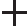
\includegraphics[scale=.9]{cross}}}
\newcommand{\crossBiColor}[2]{\raisebox{.1cm}{\pipeDreamBiColor{#1}{#2}{black}{c/l/r}}}
\newcommand{\NScross}[1][black]{\raisebox{-.15cm}{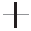
\includegraphics[scale=.9]{NScross}}}
\newcommand{\WEcross}[1][black]{\raisebox{-.15cm}{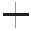
\includegraphics[scale=.9]{WEcross}}}
% elbows
%\newcommand{\elbow}[1][black]{\raisebox{.1cm}{\pipeDreamMonoColor{#1}{black}{e}}}
\newcommand{\elbow}[1][black]{\raisebox{-.15cm}{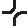
\includegraphics[scale=.9]{elbow}}}
\newcommand{\elbowBiColor}[2]{\raisebox{.1cm}{\pipeDreamBiColor{#1}{#2}{black}{e/l/r}}}
%\newcommand{\SEelbow}[1][black]{\raisebox{.1cm}{\pipeDreamBiColor{white}{#1}{black}{e/l/r}}}
\newcommand{\SEelbow}[1][black]{\raisebox{-.15cm}{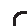
\includegraphics[scale=.9]{SEelbow}}}
%\newcommand{\WNelbow}[1][black]{\raisebox{.1cm}{\pipeDreamBiColor{#1}{white}{black}{e/l/r}}}
\newcommand{\WNelbow}[1][black]{\raisebox{-.15cm}{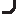
\includegraphics[scale=.9]{WNelbow}}}
\newcommand{\waving}{\mathsf{wav}}%{\raisebox{-.2cm}{\begin{tikzpicture}[scale=1]\pipeDreamBiColor{.2}{(0,0)}{black}{white}{{t/r/l},{t/l/l},{t/l/r}}\end{tikzpicture}}}
\newcommand{\transpose}{\mathsf{transp}}
\newcommand{\pipeDreams}{\Pi} % set of pipe dreams
\newcommand{\reversingPipeDreams}{\Omega} % reversing pipe dreams
\newcommand{\contact}{^\#} % contact graph
\newcommand{\se}{\textsc{se}} % southeast
\newcommand{\nw}{\textsc{nw}} % northwest
\newcommand{\duality}{^\star} % duality pipe dreams - triangulations
\newcommand{\acyclicPipeDreams}{\Sigma} % acyclic pipe dreams
\newcommand{\linearExtensions}{\mathcal{L}} % linear extensions
\newcommand{\strongLinearExtensions}{\mathcal{L}^\star} % strict linear extensions
\newcommand{\noninversions}[2]{\mathsf{ninv}(#1,#2)} % non-inversions
\newcommand{\acyclicOrientations}{\Omega} % set of pipe dreams
\newcommand{\insertion}[2]{\mathsf{pd}(#1,#2)} % insertion of permutation #1 in pipe dreams with permutation #2
\newcommand{\recoils}[2]{\mathsf{rec}(#1,#2)} % recoil scheme of a pipe dream
\newcommand{\canopy}[1]{\mathsf{can}(#1)} % canopy of a pipe dream
\newcommand{\greedyPipeDream}{P^{\overleftarrow{gr}}} % greedy facet
\newcommand{\antiGreedyPipeDream}{P^{\overrightarrow{gr}}} % antigreedy facet

% Subword complexes
\newcommand{\wo}{\omega_\circ} % longest element
\newcommand{\subwordComplex}{\mathcal{SC}} % subword complex
\newcommand{\Roots}{\mathrm{R}} % root configuration
\newcommand{\rootFunction}[2]{\mathrm{r}_{#1}(#2)} % root function
\newcommand{\subwordFacets}{\mathcal{F}} % subword complex
\newcommand{\subwordAcyclicFacets}{\mathcal{F}^\bullet} % subword complex
\newcommand{\subwordStronglyAcyclicFacets}{\mathcal{F}^\star} % subword complex
\newcommand{\greedyFacet}{I^{\overleftarrow{gr}}} % greedy facet
\newcommand{\antiGreedyFacet}{I^{\overrightarrow{gr}}} % antigreedy facet
\newcommand{\sweepingAlgorithm}{\mathsf{sweep}} % sweeping algorithm
\newcommand{\brickPolyhedron}{\mathsf{Brick}} % brick polyhedron

% lattices
\newcommand{\meet}{\wedge} % meet
\newcommand{\join}{\vee} % join
\newcommand{\less}{\vartriangleleft} % smaller WOIP
\newcommand{\more}{\vartriangleright} % larger WOIP
\newcommand{\contactLess}[1]{\less_{#1}} % smaller contact graph
\newcommand{\contactMore}[1]{\more_{#1}} % larger contact graph
\newcommand{\projDown}{\pi_\downarrow} % Down projection
\newcommand{\projUp}{\pi^\uparrow} % Down projection


%%%%%%%%%%%%%%%%%%%%%%%%%%%%%%%%%%%%%%
%%%%%%%%%%%%%%%%%%%%%%%%%%%%%%%%%%%%%%
%%%%%%%%%%%%%%%%%%%%%%%%%%%%%%%%%%%%%%

\begin{document}

\begin{abstract}
We show that for any permutation~$\omega$, the increasing flip graph on acyclic pipe dreams with exiting permutation~$\omega$ is a lattice quotient of the interval~$[e,\omega]$ of the weak order.
We then discuss conjectural generalizations of this result to acyclic facets of subword complexes on arbitrary finite Coxeter groups.
\end{abstract}

\maketitle

\tableofcontents

%%%%%%%%%%%%%%%%%%%%%%%%%%%%%%%%%%%%%%
%%%%%%%%%%%%%%%%%%%%%%%%%%%%%%%%%%%%%%
%%%%%%%%%%%%%%%%%%%%%%%%%%%%%%%%%%%%%%

\section{Introduction}
\label{sec:introduction}

The weak order is the lattice on permutations of~$[n]$ whose cover relations correspond to switching pairs of consecutive values in permutations.
The Tamari lattice is the lattice on binary trees with~$n$ internal nodes whose cover relations correspond to right rotations in binary trees.
The Tamari lattice is known to be the lattice quotient of the weak order by the sylvester congruence, defined as the equivalence relation on permutations of~$[n]$ whose equivalence classes are the sets of linear extensions of binary trees (labeled in inorder and oriented towards their leaves).

This paper develops a similar framework for acyclic pipe dreams.
Pipe dreams were introduced by N.~Bergeron and S.~Billey in~\cite{BergeronBilley} to compute Schubert polynomials and later revisited in the context of Gr\"obner geometry by A.~Knutson and E.~Miller~\cite{KnutsonMiller-GroebnerGeometry}, who coined the name \emph{pipe dreams}.
They have important connections and applications to various areas related to Schubert calculus and Schubert varieties~\cite{LascouxSchutzenberger-PolynomesSchubert, LascouxSchutzenberger-SchubertLittlewoudRichardson}. 
A pipe dream is an arrangement of pipes in the triangular shape, each entering along the vertical side and exiting along the horizontal side (see \cref{fig:pipeDreams}).
They are grouped according to their exiting permutation, given by the order in which the pipes appear along the horizontal axis.
The linear extensions of a pipe dream are the permutations of its pipes such that for each contact the northwest pipe appears before the southeast pipe in the permutation.
The pipe dreams with at least one linear extension are called acyclic and naturally appear in the study of brick polytopes~\cite{PilaudSantos-brickPolytope}.
A flip in a pipe dream exchanges a contact with a crossing between two pipes (see \cref{fig:pipeDreams}), and the flip is increasing when the contact is southwest of the crossing involved in the flip.
A brief recollection on pipe dreams is given in \cref{sec:preliminaries}.

\begin{figure}[t]
	\centerline{
		%\documentclass[10pt]{article}
\usepackage[usenames]{color} %pour la couleur
\usepackage{amssymb} %maths
\usepackage{amsmath} %maths
\usepackage[utf8]{inputenc} %utile pour taper directement les caractères accentués
\usepackage{tikz}\usetikzlibrary{trees,snakes,shapes,arrows,matrix,calc}
\usepackage{pgfplots}
\usepackage{xifthen}
\usepackage{xcolor}
\definecolor{darkgreen}{RGB}{57,181,74} % darkgreen color

\renewcommand{\b}[1]{{\color{blue} #1}} % blue
\renewcommand{\r}[1]{{\color{red} #1}} % red
\newcommand{\g}[1]{{\color{darkgreen} #1}} % green

\newcommand{\boxsize}{.35}
\newlength{\verticalOffset}
\setlength{\verticalOffset}{.3cm}
\newlength{\verticalShift}
\setlength{\verticalShift}{-.15cm}

\newcounter{length}
\newcommand{\length}[1]{%
	\setcounter{length}{0}%
	\foreach \x in {#1} {%
		\stepcounter{length}%
	}%
}

\newcommand{\pipeDreamMonoColor}[3]{% #1 = color
									% #2 = boundary color
                                    % #3 = list of types (c = cross, e = elbow, t = top, b = bottom, tb = top-bottom, or n = nothing)
	\length{#3}%
	\begin{tikzpicture}[baseline = \value{length}*\verticalShift+\verticalOffset, scale=1]
		\coordinate (origin) at (0,0);
		\newcount{\y} \y=0
		\newcount{\x}
		\foreach \line in {#3} {
			\x=0
			\foreach \t in \line {
				\coordinate (W) at ($ (origin) + ( \boxsize * \x , -\boxsize * \y ) + ( 0      , \boxsize / 2 ) $);
				\coordinate (E) at ($ (origin) + ( \boxsize * \x , -\boxsize * \y ) + ( \boxsize     , \boxsize / 2 ) $);
				\coordinate (N) at ($ (origin) + ( \boxsize * \x , -\boxsize * \y ) + ( \boxsize / 2 , \boxsize     ) $);
				\coordinate (S) at ($ (origin) + ( \boxsize * \x , -\boxsize * \y ) + ( \boxsize / 2 , 0 ) $);
				\coordinate (C) at ($ (origin) + ( \boxsize * \x , -\boxsize * \y ) + ( \boxsize / 2 , \boxsize / 2 ) $);
				\ifthenelse{\equal{\t}{e}}{
					\draw[rounded corners=\boxsize * 8, color=#1, thick] (W) -- (C) -- (N);
					\draw[rounded corners=\boxsize * 8, color=#1, thick] (S) -- (C) -- (E);			
				}{
        				\ifthenelse{\equal{\t}{c}}{
        					\draw[color=#1, thick] (W) -- (E);
        					\draw[color=#1, thick] (S) -- (N);
        				}{
        				\ifthenelse{\equal{\t}{t}}{
        					\draw[rounded corners=\boxsize * 8, color=#2] (W) -- (C) -- (N);
        					\draw[rounded corners=\boxsize * 8, color=#1, thick] (S) -- (C) -- (E);			
        				}{
        				\ifthenelse{\equal{\t}{b}}{
        					\draw[rounded corners=\boxsize * 8, color=#1, thick] (W) -- (C) -- (N);
        					\draw[rounded corners=\boxsize * 8, color=#2] (S) -- (C) -- (E);			
        				}{
        				\ifthenelse{\equal{\t}{tb}}{
        					\draw[rounded corners=\boxsize * 8, color=#2] (W) -- (C) -- (N);
        					\draw[rounded corners=\boxsize * 8, color=#2] (S) -- (C) -- (E);			
        				}{
        				\ifthenelse{\equal{\t}{n}}{}{\node at (C) {$\small \t$};}}}}}}
        				\global\advance\x by 1
			}
			\global\advance\y by 1
		}
	\end{tikzpicture}%
}

\newcommand{\pipeDreamBiColor}[4]{% #1 = colorA
                                   % #2 = colorB
                                   % #3 = boundary color
                                   % #4 = list of type/colorW/colorS (c = cross, e = elbow, or n = nothing)
	\length{#4}%
	\begin{tikzpicture}[baseline = \value{length}*\verticalShift+\verticalOffset, scale=1]
		\coordinate (origin) at (0,0);
		\newcount{\y} \y=0
		\newcount{\x}
		\foreach \line in {#4} {
			\x=0
			\foreach \t/\colorW/\colorS in \line {
				\coordinate (W) at ($ (origin) + ( \boxsize * \x , -\boxsize * \y ) + ( 0      , \boxsize / 2 ) $);
				\coordinate (E) at ($ (origin) + ( \boxsize * \x , -\boxsize * \y ) + ( \boxsize     , \boxsize / 2 ) $);
				\coordinate (N) at ($ (origin) + ( \boxsize * \x , -\boxsize * \y ) + ( \boxsize / 2 , \boxsize     ) $);
				\coordinate (S) at ($ (origin) + ( \boxsize * \x , -\boxsize * \y ) + ( \boxsize / 2 , 0 ) $);
				\coordinate (C) at ($ (origin) + ( \boxsize * \x , -\boxsize * \y ) + ( \boxsize / 2 , \boxsize / 2 ) $);
				\ifthenelse{\equal{\t}{e}}{
					\ifthenelse{\equal{\colorW}{l}}{\draw[rounded corners=\boxsize * 8, color=#1, thick] (W) -- (C) -- (N);}{}
					\ifthenelse{\equal{\colorW}{r}}{\draw[rounded corners=\boxsize * 8, color=#2, thick] (W) -- (C) -- (N);}{}
					\ifthenelse{\equal{\colorW}{b}}{\draw[rounded corners=\boxsize * 8, color=#3] (W) -- (C) -- (N);}{}
					\ifthenelse{\equal{\colorS}{l}}{\draw[rounded corners=\boxsize * 8, color=#1, thick] (S) -- (C) -- (E);}{}
					\ifthenelse{\equal{\colorS}{r}}{\draw[rounded corners=\boxsize * 8, color=#2, thick] (S) -- (C) -- (E);}{}
					\ifthenelse{\equal{\colorS}{b}}{\draw[rounded corners=\boxsize * 8, color=#3] (S) -- (C) -- (E);}{}
				}{
				\ifthenelse{\equal{\t}{c}}{
					\ifthenelse{\equal{\colorW}{l}}{\draw[color=#1, thick] (W) -- (E);}{}
					\ifthenelse{\equal{\colorW}{r}}{\draw[color=#2, thick] (W) -- (E);}{}
					\ifthenelse{\equal{\colorS}{l}}{\draw[color=#1, thick] (S) -- (N);}{}
					\ifthenelse{\equal{\colorS}{r}}{\draw[color=#2, thick] (S) -- (N);}{}
				}{
				\ifthenelse{\equal{\t}{n}}{}{\node at (C) {$\small \t$};}}}
				\global\advance\x by 1
			}
			\global\advance\y by 1
		}
	\end{tikzpicture}%
}

\newcommand{\pipeDreamTriColor}[5]{% #1 = colorA
                                   % #2 = colorB
                                   % #3 = colorC
                                   % #4 = boundary color
                                   % #5 = list of type/colorW/colorS (c = cross, e = elbow, or n = nothing)
	\length{#5}%
	\begin{tikzpicture}[baseline = \value{length}*\verticalShift+\verticalOffset, scale=1]
		\coordinate (origin) at (0,0);
		\newcount{\y} \y=0
		\newcount{\x}
		\foreach \line in {#5} {
			\x=0
			\foreach \t/\colorW/\colorS in \line {
				\coordinate (W) at ($ (origin) + ( \boxsize * \x , -\boxsize * \y ) + ( 0      , \boxsize / 2 ) $);
				\coordinate (E) at ($ (origin) + ( \boxsize * \x , -\boxsize * \y ) + ( \boxsize     , \boxsize / 2 ) $);
				\coordinate (N) at ($ (origin) + ( \boxsize * \x , -\boxsize * \y ) + ( \boxsize / 2 , \boxsize     ) $);
				\coordinate (S) at ($ (origin) + ( \boxsize * \x , -\boxsize * \y ) + ( \boxsize / 2 , 0 ) $);
				\coordinate (C) at ($ (origin) + ( \boxsize * \x , -\boxsize * \y ) + ( \boxsize / 2 , \boxsize / 2 ) $);
				\ifthenelse{\equal{\t}{e}}{
					\ifthenelse{\equal{\colorW}{l}}{\draw[rounded corners=\boxsize * 8, color=#1, thick] (W) -- (C) -- (N);}{}
					\ifthenelse{\equal{\colorW}{m}}{\draw[rounded corners=\boxsize * 8, color=#2, thick] (W) -- (C) -- (N);}{}
					\ifthenelse{\equal{\colorW}{r}}{\draw[rounded corners=\boxsize * 8, color=#3, thick] (W) -- (C) -- (N);}{}
					\ifthenelse{\equal{\colorW}{b}}{\draw[rounded corners=\boxsize * 8, color=#4] (W) -- (C) -- (N);}{}
					\ifthenelse{\equal{\colorS}{l}}{\draw[rounded corners=\boxsize * 8, color=#1, thick] (S) -- (C) -- (E);}{}
					\ifthenelse{\equal{\colorS}{m}}{\draw[rounded corners=\boxsize * 8, color=#2, thick] (S) -- (C) -- (E);}{}
					\ifthenelse{\equal{\colorS}{r}}{\draw[rounded corners=\boxsize * 8, color=#3, thick] (S) -- (C) -- (E);}{}
					\ifthenelse{\equal{\colorS}{b}}{\draw[rounded corners=\boxsize * 8, color=#4] (S) -- (C) -- (E);}{}
				}{
				\ifthenelse{\equal{\t}{c}}{
					\ifthenelse{\equal{\colorW}{l}}{\draw[color=#1, thick] (W) -- (E);}{}
					\ifthenelse{\equal{\colorW}{m}}{\draw[color=#2, thick] (W) -- (E);}{}
					\ifthenelse{\equal{\colorW}{r}}{\draw[color=#3, thick] (W) -- (E);}{}
					\ifthenelse{\equal{\colorS}{l}}{\draw[color=#1, thick] (S) -- (N);}{}
					\ifthenelse{\equal{\colorS}{m}}{\draw[color=#2, thick] (S) -- (N);}{}
					\ifthenelse{\equal{\colorS}{r}}{\draw[color=#3, thick] (S) -- (N);}{}
				}{\ifthenelse{\equal{\t}{n}}{}{\node at (C) {$\small \t$};}}}
				\global\advance\x by 1
			}
			\global\advance\y by 1
		}
	\end{tikzpicture}%
}

\begin{document}
\pipeDreamBiColor{blue}{red}{black}{
	{n,1,3,6,5,7,2,4},
	{1,e/b/l,c/l/l,c/l/l,c/l/r,c/l/l,e/l/r,e/r/b},
	{2,e/l/l,e/l/r,c/r/l,c/r/r,c/r/l,e/r/b},
	{3,e/l/r,e/r/r,c/r/l,e/r/l,e/l/b},
	{4,e/r/r,e/r/l,e/l/l,e/l/b},
	{5,e/r/l,e/l/l,e/l/b},
	{6,e/l/l,e/l/b},
	{7,e/l/b},
}
\quad
\pipeDreamBiColor{blue}{red}{black}{
	{n,1,3,6,5,7,2,4},
	{1,e/b/l,c/l/l,c/l/l,c/l/r,c/l/l,e/l/r,e/r/b},
	{2,e/l/l,e/l/r,c/r/l,e/r/r,c/r/l,e/r/b},
	{3,e/l/r,e/r/r,c/r/l,e/r/l,e/l/b},
	{4,c/r/r,e/r/l,e/l/l,e/l/b},
	{5,e/r/l,e/l/l,e/l/b},
	{6,e/l/l,e/l/b},
	{7,e/l/b},
}
\end{document}
		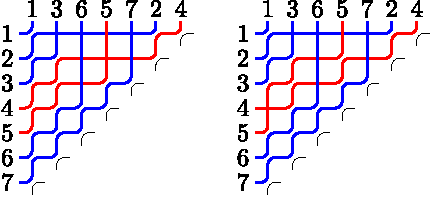
\includegraphics[scale=.9]{pipeDreams}
	}
	\caption{Two pipe dreams of~$\pipeDreams(1365724)$ connected by an increasing flip (exchanging a contact with the crossing on the two red pipes~$3$ and~$4$).}
	\label{fig:pipeDreams}
\end{figure}

In the core \cref{sec:latticeAcyclicPipeDreams} of this paper, we show that for any permutation~$\omega$,
\begin{itemize}
\item the sets of linear extensions of the acyclic pipe dreams with exiting permutation~$\omega$ form a partition of the interval~$[e,\omega]$ of the weak order (\cref{subsec:linearExtensions}),
\item the equivalence relation defined by this partition is a lattice congruence of~$[e, \omega]$, that we call the pipe dream congruence (\cref{subsec:pipeDreamCongruence}),
\item the Hasse diagram of the corresponding lattice quotient is isomorphic to the increasing flip graph on acyclic pipe dreams with exiting permutation~$\omega$ (\cref{subsec:pipeDreamQuotient}).
\end{itemize}
In summary, we obtain the following statement.

\begin{theoremA}
\label{thm:A}
For any permutation~$\omega$, the Hasse diagram of the lattice quotient of the interval~$[e,\omega]$ of the weak order by the pipe dream congruence of~$\omega$ is isomorphic to the increasing flip graph on acyclic pipe dreams with exiting permutation~$\omega$.
\end{theoremA}

Note that we recover the connection between the weak order and the Tamari lattice by the sylvester congruence for a well-chosen exiting permutation~$\omega$.

We then explore in \cref{sec:furtherTopics} some natural further topics on pipe dreams.
We describe two algorithms to compute the unique acyclic pipe dream whose linear extensions contain a given permutation generalizing the binary tree insertion map on permutations (\cref{subsec:sweepingAlgorithm,subsec:insertionAlgorithm}), we describe the pipe dream congruence as the transitive closure of a local rewriting rule generalizing that of the sylvester congruence (\cref{subsec:rewritingRule}), and we describe a natural commutative diagram of lattice morphism generalizing the connection between the recoil map and the binary tree insertion map on permutations and the canopy on binary trees (\cref{subsec:canopy}).

Finally, we discuss in \cref{sec:subwordComplexes} (partly conjectural) extensions of our results to subword complexes in finite Coxeter groups~\cite{KnutsonMiller-subwordComplex}.
Given a finite Coxeter group~$W$ with simple reflections~$S$, a word~$Q$ on~$S$ and an element~$\omega$ of~$W$, the subword complex~$\subwordComplex(Q,\omega)$ is a simplicial complex whose facets are the complements of the reduced expressions of~$\omega$ inside the word~$Q$.
Pipe dreams can be seen as facets of subword complexes for special words~$Q$ on the simple transpositions of the symmetric groups.
In general, there is again a natural increasing flip graph on the facets of a subword complex, which was studied in particular in~\cite{PilaudStump-ELlabelings}.
An important tool to understand this flip is the root function introduced in~\cite{CeballosLabbeStump}, which associates a root~$\rootFunction{I}{i}$ to each position~$i$ and each facet~$I$, and the root configuration~$\Roots(I)$ of a facet~$I$, which collects all roots~$\rootFunction{I}{i}$ at positions~$i$ in~$I$.
A brief recollection on finite Coxeter systems and subword complexes is given in \cref{subsec:finiteCoxeterGroups,subsec:subwordComplexes}.

We consider the set~$\linearExtensions(I)$ of linear extensions of a facet~$I$ of~$\subwordComplex(Q,\omega)$, that is the set of elements~$\pi$ of~$W$ such that~${\Roots(I) \subseteq \pi(\Phi^+)}$.
We prove the following statement in \cref{subsec:twoTheorems}.

\begin{theoremA}
\label{thm:B}
For any non-empty subword complex~$\subwordComplex(Q, \omega)$, the sets~$\linearExtensions(I)$ for all facets~$I$ of~$\subwordComplex(Q, \omega)$ are order convex and form a partition of a lower set of the weak order that contains the interval~$[e, \omega]$.
\end{theoremA}

In contrast to the case of pipe dreams, there are some subword complexes and some facets for which the interval~$[e, \omega]$ does not contain (even sometimes does not intersect) the set of linear extensions~$\linearExtensions(I)$.
However, there is a large family of subword complexes for which this cannot happen.
We say that~$Q$ is sorting if it contains a reduced expression for~$\wo$.

\begin{theoremA}
\label{thm:C}
If~$Q$ is sorting, then the sets~$\linearExtensions(I)$ for all facets~$I$ of~$\subwordComplex(Q, \omega)$ form a partition of the interval~$[e, \omega]$.
\end{theoremA}

In the case when~$[e, \omega]$ does not contain all sets of linear extensions, it is natural to consider the restriction of this partition to~$[e, \omega]$ by the sets~$[e, \omega] \cap \linearExtensions(\omega)$.
This defines an equivalence relation~$\equiv_{Q, \omega}$ on~$[e, \omega]$ that we call the subword complex congruence.
However, as the sets of linear extensions are not always intervals of the weak order, this equivalence relation is not always a lattice congruence.
This seems to be fixed by an additional assumption on~$Q$.
We say that~$Q$ is alternating when all non-commuting pairs $s, t\in S$ alternate within $Q$ (this notion was already considered in \cite{PilaudSantos-brickPolytope, CeballosLabbeStump}).

\begin{conjectureA}
\label{conj:A}
If~$Q$ is alternating, then the subword complex congruence~$\equiv_{Q, \omega}$ is a lattice congruence of the interval~$[e, \omega]$ of the weak order.
\end{conjectureA}

When~$Q$ is alternating, we can thus consider the quotient~$[e, \omega]/{\equiv_{Q, \omega}}$.
In contrast to the case of pipe dreams, the Hasse diagram of the quotient~$[e, \omega]/{\equiv_{Q, \omega}}$ is not always isomorphic to the increasing flip graph on acyclic facets of~$\subwordComplex(Q, \omega)$ for two reasons:
\begin{itemize}
\item First, not all acyclic facets of~$\subwordComplex(Q, \omega)$ appear as vertices of~$[e, \omega]/{\equiv_{Q, \omega}}$ (see \cref{rem:linearExtensionsPartitionSubwordComplexA}). We say that a facet is strongly acyclic if~$[e, \omega] \cap \linearExtensions(\omega) \ne \varnothing$.
\item Second, not all flips between two strongly acyclic facets of~$\subwordComplex(Q, \omega)$ define a cover relation of~$[e, \omega]/{\equiv_{Q, \omega}}$ (see \cref{exm:acyclicFlipvsWeakOrder}). We say that the flip of a position~$i$ in a facet~$I$ is external if the root~$\rootFunction{I}{i}$ directing the flip is a ray of the root configuration~$\Roots(I)$.
\end{itemize}
This leads us to the following conjecture.

\begin{conjectureA}
\label{conj:B}
If~$Q$ is alternating, then the Hasse diagram of the quotient~$[e, \omega]/\equiv_{Q, \omega}$ is isomorphic to the graph of extremal increasing flips between strongly acyclic facets of~$\subwordComplex(Q, \omega)$.
\end{conjectureA}

Combining the sorting and alternating conditions of \cref{thm:B,conj:A,conj:B}, we thus obtain the following conjecture, which can be seen as the natural extension of~\cref{thm:A}.

\begin{conjectureA}
\label{conj:C}
If~$Q$ is sorting and alternating, then the Hasse diagram of the quotient~$[e, \omega]/\equiv_{Q, \omega}$ is isomorphic to the graph of extremal increasing flips between acyclic facets of~$\subwordComplex(Q, \omega)$.
\end{conjectureA}

This last conjecture has a strong connection to the geometry of subword complexes given by brick polytopes~\cite{PilaudSantos-brickPolytope, PilaudStump-brickPolytope} and brick polyhedra~\cite{JahnStump}.
Namely, the extremal increasing flips between acyclic facets of~$\subwordComplex(Q, \omega)$ is precisely the bounded part (meaning forgetting the unbounded rays) of the brick polyhedron~$\brickPolyhedron(Q, \omega)$ oriented by a natural linear functional.
\cref{conj:C} thus translates geometrically to the following.

\begin{conjectureA}
\label{conj:D}
If~$Q$ is sorting and alternating, then the oriented graph of the brick polyhedron~$\brickPolyhedron(Q, \omega)$ is isomorphic to the Hasse diagram of the lattice quotient~$[e, \omega]/\equiv_{Q, \omega}$.
\end{conjectureA}

In particular, when~$\omega = \wo$, we obtain the following conjecture, extending results from~\cite{Pilaud-brickAlgebra}.

\begin{conjectureA}
\label{conj:E}
If~$Q$ is sorting and alternating, then the oriented graph of the brick polytope $\brickPolyhedron(Q, \wo)$ is isomorphic to the Hasse diagram of the lattice quotient of the weak order by~$\equiv_{Q, \omega}$.
\end{conjectureA}

%%%%%%%%%%%%%%%%%%%%%%%%%%%%%%%%%%%%%%
%%%%%%%%%%%%%%%%%%%%%%%%%%%%%%%%%%%%%%
%%%%%%%%%%%%%%%%%%%%%%%%%%%%%%%%%%%%%%

\section{Preliminaries on pipe dreams}
\label{sec:preliminaries}

% Let $\fS_n$ denote the set of permutations of~$[n] \eqdef \{1,2,\ldots,n\}$, and let~$\fS \eqdef \bigsqcup_{n \ge 0} \fS_n$.

%%%%%%%%%%%%%%%%%%%%%%%%%%%%%%%%%%%%%%

\subsection{Pipe dreams}
\label{subsec:pipeDreams}

A \defn{pipe dream}~$P$ is a filling of a triangular shape with crossings~\cross{} and contacts~\elbow{} so that all pipes entering on the left side exit on the top side.
We only consider \defn{reduced} pipe dreams, where two pipes have at most one crossing.
We label the pipes with~$1, 2, \dots, n$ in the order of their entry points from top to bottom.
We denote by~$\omega_P \in \fS_n$ the order of the exit points of the pipes of~$P$ from left to right.
In other words, the pipe entering at row~$i$ exits at column~$\omega^{-1}_P(i)$.
For a fixed permutation~$\omega \in \fS_n$, we denote by~$\pipeDreams(\omega)$ the set of reduced pipe dreams~$P$ such that~$\omega_P = \omega$.
% We let~$\pipeDreams_n \eqdef \bigsqcup_{\omega \in \fS_n} \pipeDreams(\omega)$ and~$\pipeDreams \eqdef \bigsqcup_{n \in \N} \pipeDreams_n$.

%Two pipe dreams are related by a \defn{flip} if they only differ by the position of a crossing and a contact (in particular, they define the same permutation).
A contact~$c$ is \defn{flippable} if the two pipes passing through contact~$c$ have a crossing~$x$.
The \defn{flip} exchanges the contact~$c$ with the crossing~$x$.
%See \cref{fig:pipeDreams}.
The flip is \defn{increasing} if the contact~$c$ is weakly southwest of the crossing~$x$.
For example, \cref{fig:pipeDreams} illustrates an increasing flip from the left pipe dream to the right pipe dream.
%
The \defn{increasing flip graph} is the graph of increasing flips on~$\pipeDreams(\omega)$.
It is clearly a directed acyclic graph, and it has a unique source and a unique sink \cite{PilaudPocchiola}, called the \defn{greedy} and \defn{antigreedy} pipe dreams, and denoted~$\greedyPipeDream$ and~$\antiGreedyPipeDream$.
\vincent{In \cite{PilaudStump-ELlabelings}, these are called positive and negative greedy facets. Also the notations are different...}
The \defn{increasing flip poset} is the reflexive and transitive closure of the increasing flip graph on~$\pipeDreams(\omega)$.

The \defn{contact graph} of a pipe dream~$P$ is the directed graph~$P\contact$ with one node for each pipe of~$P$ and one arc for each contact of~$P$ connecting the northwest pipe to the southeast pipe of the contact\footnote{We have reversed the usual orientation conventions of \cite{PilaudSantos-brickPolytope, PilaudPocchiola, Pilaud-brickAlgebra} to suit better our purposes, in particular in \cref{subsec:insertionAlgorithm}.}.
We see equivalently the contact graph~$P\contact$ as a (multi)graph on the pipes of~$P$ or on the integers~$[n]$.
We say that a pipe dream~$P$ is \defn{acyclic} if its contact graph~$P\contact$ has no oriented cycle.
For an acyclic pipe dream~$P$, we denote by~$\contactLess{P}$ the transitive closure of the contact graph of~$P$.
For~$\omega \in \fS_n$, we denote by~$\acyclicPipeDreams(\omega)$ the set of acyclic pipe dreams of~$\pipeDreams(\omega)$.
% We let~$\acyclicPipeDreams_n \eqdef \bigsqcup_{\omega \in \fS_n} \acyclicPipeDreams(\omega)$ and~$\acyclicPipeDreams \eqdef \bigsqcup_{n \in \N} \acyclicPipeDreams_n$.
%\vincent{Add contact graphs to \cref{fig:pipeDreams}.}

\begin{example}
\label{exm:Tamari1}
We say that a pipe dream is \defn{reversing} if it fixes the first and last pipes and reverses the order of the remaining pipes.
In this case, it is natural to label the pipes from~$0$ to~$n+1$, so that the permutation of the pipes is~$\rho_n \eqdef [0, n, n-1, \dots, 2, 1, n+1]$.
% We denote by~$\reversingPipeDreams_n$ the reversing pipe dreams of~$\pipeDreams_n$.
As observed in~\cite{Woo, PilaudPocchiola, Pilaud-these, Stump}, the family of reversing pipe dreams belong to the Catalan families, meaning that it is counted by the famous Catalan numbers.
\cref{fig:bijection} illustrates explicit bijections between reversing pipe dreams of~$\pipeDreams(\rho_n)$, binary trees with $n$ internal nodes, and the triangulations of a convex $(n+2)$-gon.
More precisely, the map which sends a contact in row~$i$ and column~$j$ of the triangular shape (indexed from~$0$ to~$n+1$) to the diagonal~$[i,n+1-j]$ of the~$(n+2)$-gon provides the following correspondence: \\[.3cm]
\centerline{
\begin{tabular}{r@{$\quad\longleftrightarrow\quad$}l}
pipe dream~$P \in \reversingPipeDreams_n$ & triangulation~$P\duality$ of the $(n+2)$-gon, \\
pipe $i$ of~$P$ & triangle $i\duality$ of~$P\duality$ (with central vertex~$i$), \\
contact between pipes~$i$ and~$j$ of~$P$ & common side of triangles~$i\duality$ and~$j\duality$ of~$P\duality$, \\
crossing between pipes~$i$ and~$j$ of~$P$ & common bisector of triangles~$i\duality$ and~$j\duality$ of~$P\duality$, \\
contact graph of~$P$ & dual binary tree of~$P\duality$, \\
contact flips in~$P$ & diagonal flips in~$P\duality$. \\
%increasing flip poset & Tamari lattice.
\end{tabular}} \\[.3cm]
%
\begin{figure}
	\centerline{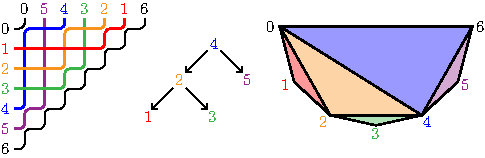
\includegraphics[scale=1.3]{dualiteTriangulation}}
	\caption{The bijection between reversing pipe dreams (left), binary trees (middle) and triangulations (right).}
	\label{fig:bijection}
\end{figure}
%
As a consequence, this map sends the increasing flip poset on reversing pipe dreams to the \defn{Tamari lattice} on binary trees.
This lattice is defined as the transitive closure of right rotations on binary trees, and is obtained as the quotient of the weak order by the \defn{sylvester congruence}.
An important point here is that all reversing pipe dreams are acyclic, since there contact graphs are (oriented) binary trees.
\end{example}

%%%%%%%%%%%%%%%%%%%%%%%%%%%%%%%%%%%%%%

\subsection{Crossing and contact properties}
\label{subsec:crossingsContacts}

We now gather some elementary properties of crossings and contacts in pipe dreams that will be needed later to construct pipe dreams from permutations.
For a pipe dream~$P \in \pipeDreams(\omega)$, we call pipe~$j$ the pipe which enters at row~$j$ and exits at column~$\omega^{-1}(j)$.

\begin{lemma}
\label{lem:horiVertCrossings}
For any pipe dream~$P \in \pipeDreams(\omega)$, the pipe~$j$ of~$P$ crosses precisely
\begin{itemize}
\item vertically the pipes~$i$ such that~$i < j$ while~$\omega^{-1}(i) > \omega^{-1}(j)$,
\item horizontally the pipes~$k$ such that~$j < k$ while~$\omega^{-1}(j) > \omega^{-1}(k)$.
\end{itemize}
\end{lemma}

\begin{proof}
For~$i < j$, if~$\omega^{-1}(i) > \omega^{-1}(j)$, then the pipes~$i$ and~$j$ have to cross exactly once (and $j$ must be the vertical pipe at that crossing), while if~$\omega^{-1}(i) < \omega^{-1}(j)$ the pipes~$i$ and~$j$ cannot cross.
The same argument applies for~${k > j}$.
\end{proof}

\begin{lemma}
\label{lem:countingElbows}
For any pipe dream~$P \in \pipeDreams(\omega)$, the pipe~$j$ has precisely
\begin{itemize}
\item $\noninversions{\omega}{j}$ many southeast elbows\!\SEelbow{}
\item $1+\noninversions{\omega}{j}$ many northwest elbows~\WNelbow{}
\item $j-1-\noninversions{\omega}{j}$ vertical crossings~\NScross
\item $\omega^{-1}(j)-1-\noninversions{\omega}{j}$ horizontal crossings~\WEcross
\end{itemize}
where~$\noninversions{\omega}{j} \eqdef \#\set{i \in [n]}{i < j \text{ and } \omega^{-1}(i) < \omega^{-1}(j)}$.
\end{lemma}

\begin{proof}
Pipe~$j$ enters at row~$j$ and exits at column~$\omega^{-1}(j)$, so that it passes through~$j+\omega^{-1}(j)-1$ grid points.
By \cref{lem:horiVertCrossings}, it has~$\#\set{i \in [n]}{i < j \text{ and } \omega^{-1}(i) > \omega^{-1}(j)} = j-1-\noninversions{\omega}{j}$ vertical crossings and~$\#\set{k \in [n]}{j < k \text{ and } \omega^{-1}(j) > \omega^{-1}(k)} = \omega^{-1}(j)-1-\noninversions{\omega}{j}$ horizontal crossings.
The~$1+2\,\noninversions{\omega}{j}$ remaining grid points along the pipe~$j$ are thus alternating northwest elbows and southeast elbows.
\end{proof}

\begin{lemma}
\label{lem:characterizationPipeDreams}
A collection~$P$ of~$n$ pipes pairwise disjoint except at crossing and contacts and such that for each~$j \in [n]$, the pipe~$j$ enters at row~$j$, exits at column~$\omega^{-1}(j)$, and has~$\noninversions{\omega}{j}$ southeast contacts is a pipe dream of~$\pipeDreams(\omega)$.
\end{lemma}

\begin{proof}
The argument is similar to the previous lemma.
Observe first that the pipe~$j$ must cross the paths~$i$ such that~$i < j$ and~$\omega^{-1}(i) > \omega^{-1}(j)$ and the paths~$k$ such that~$j < k$ and~$\omega^{-1}(j) > \omega^{-1}(k)$.
Moreover, it has~$\noninversions{\omega}{j}$ southeast elbows and thus~$1+\noninversions{\omega}{j}$ northwest elbows.
This already exhausts all~$j+\omega^{-1}(j)-1$ grid points of~$j$.
Therefore, the pipe~$j$ can only cross at most once any other pipe.
\end{proof}

%%%%%%%%%%%%%%%%%%%%%%%%%%%%%%%%%%%%%%

\subsection{Contact graph properties}
\label{subsec:contactGraph}

We now state a simple observation about the poset~$\contactLess{P}$, and two of its consequences, that will play essential roles in the proofs in \cref{sec:latticeAcyclicPipeDreams}.

\begin{lemma}
\label{lem:rectangle}
Let~$P$ be a pipe dream and~$i,j$ be pipes of~$P$.
If there is an elbow of pipe~$i$ weakly northwest of an elbow of pipe~$j$, then~$i \contactLess{P} j$.
\end{lemma}

\begin{proof}
Let~$x$ (resp.~$y$) be the location of an elbow of pipe~$i$ (resp.~$j$) such that~$x$ is weakly northwest of~$y$.
We proceed by induction on the grid distance from~$x$ to~$y$.
If they coincide, then pipes~$i$ and~$j$ share a contact, so that there is an edge from~$i$ to~$j$ in~$P\contact$.
Otherwise, let~$k$ be the pipe of~$P$ with a southeast elbow at~$x$ ($k$ is either the pipe~$i$ itself, or there is an edge from~$i$ to~$k$ in~$P\contact$) and~$\ell$ be the pipe of~$P$ with a northwest elbow at~$y$ ($\ell$ is either the pipe~$j$ itself, or there is an edge from~$\ell$ to~$j$ in~$P\contact$).
Let~$R$ be the axis-parallel rectangle with corners~$x$ and~$y$.
Since pipes~$k$ and~$\ell$ cross at most once, at least one of them has an additional elbow along the sides of~$R$.
Assume for instance that~$k$ has an elbow at~$x'$.
Then~$x'$ is still weakly northwest of~$y$ and $x',y$ are strictly closer than~$x,y$.
By induction, there is a directed path from~$k$ to~$\ell$ in~$P\contact$, and thus a path directed form~$i$ to~$j$.
\end{proof}

Note that the reciprocal assertion of \cref{lem:rectangle} is false.
We conclude this section by two consequences of \cref{lem:rectangle}.

\begin{lemma}
\label{lem:consequenceRectangle1}
If~$i < j$ and~$\omega^{-1}(i) < \omega^{-1}(j)$, then $i \contactLess{P} j$ for any~$P \in \pipeDreams(\omega)$.
\end{lemma}

\begin{proof}
If~$i < j$ and~$\omega^{-1}(i) < \omega^{-1}(j)$, then the pipes~$i$ and~$j$ do not cross.
Consider an elbow~$e$ of the pipe~$i$.
Since the pipe~$j$ passes southeast of~$e$, it has an elbow southeast of~$e$.
We conclude that~$i \contactLess{P} j$ by \cref{lem:rectangle}.
\end{proof}

\begin{lemma}
\label{lem:consequenceRectangle2}
Let~$P$ be a pipe dream and let~$i,j,k$ be three pipes of~$P$ such that~$i < j < k$ and~$\omega^{-1}(i) > \omega^{-1}(j) > \omega^{-1}(k)$.
If~$i \to k$ in~$P\contact$, then either~$i \contactLess{P} j \contactMore{P} k$ or~$i \contactMore{P} j \contactLess{P} k$.
\end{lemma}

\begin{proof}
Let~$c$ denote the contact of pipes~$i$ and~$k$ in~$P$.
Decompose the triangular shape into three regions: the region~$A$ of all points located southwest of~$c$, the region~$B$ of all points located northwest or southeast of~$c$, and the region~$C$ of all points located northeast of~$c$.
Since~$i < j$ and~$\omega^{-1}(j) > \omega^{-1}(k)$, the pipe~$j$ starts in region~$A$ and ends in region~$C$.
Hence, the pipe~$j$ has an elbow~$e$ in region~$B$.
We thus obtain that~$i \contactLess{P} j \contactMore{P} k$ if this $e$ is southeast of~$c$, and that~$i \contactMore{P} j \contactLess{P} k$ if $e$ is northwest of~$c$.
\end{proof}

%\begin{lemma}
%\label{lem:consequenceRectangle2}
%Let~$P$ be a pipe dream and let~$i,j,k$ be three pipes of~$P$ such that~$\min(i,k) < j$ and~$\min(\omega^{-1}(i), \omega^{-1}(k)) < \omega^{-1}(j)$.
%If~$i \to k$ in~$P\contact$, then either~$i \contactLess{P} j \contactMore{P} k$ or~$i \contactMore{P} j \contactLess{P} k$.
%\vincent{not sure we really use this extended version}
%\end{lemma}
%
%\begin{proof}
%Let~$e$ denote the contact of pipes~$i$ and~$k$ in~$P$.
%Decompose the triangular shape into three regions: the region~$A$ of all points located southwest of~$e$, the region~$B$ of all points located northwest or southeast of~$e$, and the region~$C$ of all points located northeast of~$e$.
%Since~$\min(i,k) < j$ and~$\min(\omega^{-1}(i), \omega^{-1}(k)) < \omega^{-1}(j)$, the pipe~$j$ starts in region~$A$ and ends in region~$C$.
%Hence, the pipe~$j$ has a contact~$f$ in region~$B$.
%We thus obtain that~$i \contactLess{P} j \contactMore{P} k$ if this $f$ is southeast of~$e$, and that~$i \contactMore{P} j \contactLess{P} k$ if $f$ is northwest of~$e$.
%\end{proof}

%%%%%%%%%%%%%%%%%%%%%%%%%%%%%%%%%%%%%%
%%%%%%%%%%%%%%%%%%%%%%%%%%%%%%%%%%%%%%
%%%%%%%%%%%%%%%%%%%%%%%%%%%%%%%%%%%%%%

\section{Lattice of acyclic pipe dreams}
\label{sec:latticeAcyclicPipeDreams}

As already mentioned, the increasing flip poset on reversing pipe dreams is isomorphic to the Tamari lattice, which is a lattice quotient of the weak order.
In this section, we extend this result to any permutation~$\omega$ by showing that the sets of linear extensions of pipe dreams of~$\acyclicPipeDreams(\omega)$ partition the interval~$[e,w]$ (\cref{subsec:linearExtensions}), that this partition actually defines a lattice congruence of the weak order on~$[e,w]$ (\cref{subsec:pipeDreamCongruence}), and that the Hasse diagram of the quotient by this congruence is the increasing flip graph on acyclic pipe dreams of~$\acyclicPipeDreams(\omega)$ (\cref{subsec:pipeDreamQuotient}).
This section goes straight to the proof of this property, and leaves alternative perspectives on this quotient to \cref{sec:furtherTopics}.

%%%%%%%%%%%%%%%%%%%%%%%%%%%%%%%%%%%%%%

\subsection{Linear extensions of pipe dreams}
\label{subsec:linearExtensions}

The main characters in this section are the following sets of permutations.

%Recall that a \defn{linear extension} of a binary relation~$\less$ on~$[n]$ is a permutation~$\pi \in \fS_n$ such that~$i \less j$ implies $\pi^{-1}(i) < \pi^{-1}(j)$.
%We denote by~$\linearExtensions(\less)$ the set of linear extensions of~$\less$.
%Consider an acyclic pipe dream~$P$, and recall that we denote by~$\contactLess{P}$ the transitive closure of the contact graph~$P\contact$ of~$P$.
%We denote by~$\linearExtensions(P)$ the set of linear extensions of~$\contactLess{P}$, and we say abusively that the permutations of~$\linearExtensions(P)$ are linear extensions of~$P$.
%In other words, $\pi \in \linearExtensions(P)$ if and only if~$\pi^{-1}(i) < \pi^{-1}(j)$ for all arcs~$i \to j$ in~$P\contact$.

\begin{definition}
\label{def:linearExtensions}
We say that a permutation~$\pi$ is a \defn{linear extension} of a pipe dream~$P \in \pipeDreams(\omega)$ if~$\pi^{-1}(i) < \pi^{-1}(j)$ for every arc~$i \to j$ in~$P\contact$ (we should say linear extension of~$\contactLess{P}$, but prefer to simplify notation).
We denote by~$\linearExtensions(P)$ the set of linear extensions of~$P$.
%For a pipe dream~$P \in \pipeDreams(\omega)$, we denote by~$\linearExtensions(P)$ the set of \defn{linear extensions} of~$P$, \ie the permutations~$\pi$ of~$[n]$ such that~$\pi^{-1}(i) < \pi^{-1}(j)$ for every arc~$i \to j$ in~$P\contact$.
\end{definition}

In this section, we prove the following structural property of~$\linearExtensions(P)$.

\begin{theorem}
\label{thm:partitionPipeDreams}
The set~$\set{\linearExtensions(P)}{P \in \acyclicPipeDreams(\omega)}$ partitions the weak order interval~$[e,\omega]$.
\end{theorem}

\begin{example}
\label{exm:Tamari2}
Following \cref{exm:Tamari1}, observe that the permutations of~$\{0, 1, \dots, n, n+1\}$ below $\rho_n$ are precisely the permutations of the form~$[0, \pi, n+1]$ for some~$\pi \in \fS_n$.
It is well-known that any permutation~$\pi \in \fS_n$ is a linear extension of a unique binary tree.
This binary tree can be obtained by inserting~$\pi$ from right to left in a binary search tree.
Hence any permutation of~$\{0, 1, \dots, n, n+1\}$ below~$\rho_n$ is a linear extension of a unique reversing pipe dream on~$n+2$ pipes.
For instance, the pipe dream of \cref{fig:bijection} has linear extensions~$0421356$, $0423156$, $0421536$, $0423516$, $0425136$, $0425316$, $0452136$, $0452316$.
\end{example}

We will see in \cref{sec:furtherTopics} insertion algorithms to compute the pipe dream~$P \in \acyclicPipeDreams(\omega)$ such that~$\pi \in \linearExtensions(P)$ for given permutations~$\pi < \omega$.
These algorithms are however not needed for the proof of \cref{thm:partitionPipeDreams}, which we break into the following three lemmas.

\begin{lemma}
\label{lem:lowerSetPipeDreams}
If~$\pi \eqdef UjiV$ covers $\pi' \eqdef UijV$ in weak order, and ${\pi \in \linearExtensions(P)}$ for some~${P \in \acyclicPipeDreams(\omega)}$,~then
\begin{itemize}
\item if~$P\contact$ has no arc~$j \to i$, then~$\pi' \in \linearExtensions(P)$,
\item otherwise, $\pi' \in \linearExtensions(P')$ where~$P'$ denotes the pipe dream obtained from~$P$ by flipping the furthest northeast contact between pipes~$i$ and~$j$ in~$P$.
\end{itemize}
\end{lemma}

\begin{proof}
The first point is obvious.
For the second point, observe that the flip of the furthest contact just reverses all arcs~$j \to i$ and exchanges~$i$ and~$j$ at some extremities of the arcs of the contact graph.
\end{proof}

\begin{lemma}
\label{lem:partition}
If~$\pi \le \omega$ in weak order, then~$\pi$ is a linear extension of a unique pipe dream~$P \in \acyclicPipeDreams(\omega)$.
\end{lemma}

\begin{proof}
Consider the greedy and antigreedy pipe dreams~$\greedyPipeDream$ and~$\antiGreedyPipeDream$ of \cite{PilaudPocchiola}.
For any contact between the pipes~$i$ and~$j$ in~$\greedyPipeDream$, with~$i < j$, we have
\begin{itemize}
\item if the pipes~$i$ and~$j$ never cross, then~$\omega^{-1}(i) < \omega^{-1}(j)$,
\item if the pipes~$i$ and~$j$ cross, then~$\omega^{-1}(i) > \omega^{-1}(j)$ and the contact in~$\greedyPipeDream$ must be from~$i$ to~$j$ (since all flips in~$\greedyPipeDream$ are increasing by definition).
\end{itemize}
We conclude that~$e \in \linearExtensions(\greedyPipeDream)$.
Conversely, if~$e \in \linearExtensions(P)$, all arcs of~$P\contact$ are increasing, so that all flips in~$P$ are increasing.
We conclude that~$\greedyPipeDream$ is the unique pipe dream with~$e \in \linearExtensions(\greedyPipeDream)$.
Similar arguments show that~$\antiGreedyPipeDream$ is the unique pipe dream with~$\omega \in \linearExtensions(\antiGreedyPipeDream)$.
The result thus follows from~\cref{lem:lowerSetPipeDreams}, since it shows that the existence (resp.~uniqueness) of a pipe dream~$P$ such that~$\pi \in \linearExtensions(P)$ is preserved when going down (resp.~up) in weak order.
\end{proof}

\begin{lemma}
\label{lem:interval}
If~$\pi$ is a linear extension of a pipe dream~$P \in \acyclicPipeDreams(\omega)$, then~$\pi \le \omega$ in weak order.
\end{lemma}

\begin{proof}
For any~$i < j$ with~$\omega^{-1}(i) < \omega^{-1}(j)$, we have~$i \contactLess{P} j$ by \cref{lem:consequenceRectangle1}, thus ${\pi^{-1}(i) < \pi^{-1}(j)}$ since~$\pi \in \linearExtensions(P)$.
In other words, any non-inversion of~$\omega$ is a non-inversion of~$\pi$, so that~${\pi \le \omega}$.
\end{proof}

\begin{proof}[Proof of \cref{thm:partitionPipeDreams}]
Direct consequence of \cref{lem:partition,lem:interval}.
\end{proof}

\begin{notation}
For~$\pi \in [e, \omega]$, we denote by~$\insertion{\pi}{\omega}$ the pipe dream of~$\acyclicPipeDreams(\omega)$ such that~${\pi \in \linearExtensions(\insertion{\pi}{\omega})}$.
\end{notation}

%%%%%%%%%%%%%%%%%%%%%%%%%%%%%%%%%%%%%%

\subsection{Pipe dream congruence}
\label{subsec:pipeDreamCongruence}

A \defn{congruence} of a lattice~$(L, \le, \meet, \join)$ is an equivalence relation~$\equiv$ on~$L$ which respects meets and joins: $x \equiv x'$ and~$y \equiv y'$ implies $x \meet y \equiv x' \meet y'$ and~$x \join y \equiv x' \join y'$.
We will use the following classical characterization of lattice congruences, see~\cite{Reading-PosetRegionsChapter}.

\begin{proposition}
\label{prop:characterizationCongruences}
An equivalence relation~$\equiv$ on a lattice~$L$ is a congruence if and only if
\begin{enumerate}[(i)]
\item every equivalence class of~$\equiv$ is an interval of~$L$,
\item the projections~$\projDown : L \to L$ and~$\projUp : L \to L$, which maps an element of~$L$ to the minimal and maximal elements of its equivalence class respectively, are order preserving.
\end{enumerate}
\end{proposition}

We now focus on the following congruence.

\begin{definition}
\label{def:pipeDreamCongruence}
The \defn{pipe dream congruence} is the equivalence relation~$\equiv_\omega$ on the weak order interval~$[e,\omega]$ whose equivalence classes are the sets~$\linearExtensions(P)$ of linear extensions of the pipe dreams~$P$ of~$\acyclicPipeDreams(\omega)$.
In other words, $\pi \equiv_\omega \pi'$ if and only if~$\insertion{\pi}{\omega} = \insertion{\pi'}{\omega}$.
\end{definition}

Note that the pipe dream congruence indeed defines an equivalence relation by \cref{thm:partitionPipeDreams}.
In this section, we prove that it is a lattice congruence.

\begin{theorem}
\label{thm:pipeDreamCongruence}
The pipe dream congruence~$\equiv_\omega$ is a congruence of the weak order interval~$[e,\omega]$.
\end{theorem}

\begin{example}
\label{exm:Tamari3}
Following \cref{exm:Tamari1,exm:Tamari2}, observe that the congruence~$\equiv_{\rho_n}$ on the permutations of~$\{0, 1, \dots, n, n+1\}$ below~$\rho_n$ corresponds to the sylvester congruence on~$\fS_n$.
The classes of this congruence are the sets of linear extensions of the binary trees (considered as posets, labeled in inorder, and oriented towards their roots).
It can also be defined by the classical rewriting rule~$UjVikW \equiv UjVkiW$ where~$i < j < k$ are elements of~$[n]$ while~$U, V, W$ are (possibly empty) words on~$[n]$.
\end{example}

We will discuss in \cref{subsec:rewritingRule} rewriting rules for the pipe dream congruence~$\equiv_\omega$, for any permutation~$\omega$.
These rewriting rules are however not needed for the proof of \cref{thm:pipeDreamCongruence}.
We prove it by checking both conditions of \cref{prop:characterizationCongruences}.
For the first condition, we need the following classical characterization of weak order intervals, see \cite{BjornerWachs} or~\cite{ChatelPilaudPons}.

\begin{proposition}[{\cite[Thm.~6.8]{BjornerWachs}}]
\label{prop:WOIP}
The set~$\linearExtensions(\less)$ of linear extensions of a poset~$\less$ on~$[n]$ forms an interval~$I$ of the weak order if and only if for every~$i < j < k$,
\[
i \less k \implies i \less j \text{ or } j \less k
\qquad\text{and}\qquad
i \more k \implies i \more j \text{ or } j \more k.
\]
Moreover, the inversions of~$\min(I)$ are the pairs~$i,j \in [n]$ with $i < j$ and $i \more j$, and the non-inversions of~$\max(I)$ are the pairs~$i,j \in [n]$ with $i < j$ and $i \less j$.
\end{proposition}

\begin{proposition}
\label{prop:intervals}
For any pipe dream~$P \in \acyclicPipeDreams(\omega)$, the set~$\linearExtensions(P)$ is an interval of the weak order.
\end{proposition}

\begin{proof}
We just need to show that the poset~$\contactLess{P}$ satisfies the conditions of \cref{prop:WOIP}.
Consider~$i < j < k$ such that~$i \contactLess{P} k$.
If~$\omega^{-1}(i) < \omega^{-1}(j)$, then~$i \contactLess{P} j$ by \cref{lem:consequenceRectangle1}.
Similarly, if~$\omega^{-1}(j) < \omega^{-1}(k)$, then~$j \contactLess{P} k$ by \cref{lem:consequenceRectangle1}.
We can thus assume that~${\omega^{-1}(i) > \omega^{-1}(j) > \omega^{-1}(k)}$.
Decompose the triangular shape into three regions: the region~$A$ of all points located northeast of the last elbow of the pipe~$j$ of~$P$, the region~$B$ of all points located northwest or southeast of an elbow of the pipe~$j$ of~$P$, and the region~$C$ of all points located southwest of the first elbow of the pipe~$j$ of~$P$.
Since~$i \contactLess{P} k$, there is a path~$\pi$ form the exiting point of the pipe~$i$ of~$P$ to the entering point of the pipe~$j$ of~$P$ which travels along the pipes of~$P$, possibly jumping from the northwest pipe to the southeast pipe of a contact it encounters.
Since~$i < j$ and~$\omega^{-1}(j) > \omega^{-1}(k)$, the path~$\pi$ starts in region~$A$ and ends in region~$C$, so that it necessarily passes from region~$A$ to region~$C$.
Since the southwest corner of~$A$ is located northeast of the northeast corner of~$C$, this forces an elbow~$e$ of~$\pi$ to lie in region~$B$.
\cref{lem:rectangle} then ensures that either~$i \contactLess{P} j$ (if~$e$ is north of pipe~$j$), or~$j \contactLess{P} k$ (if~$e$ is south of pipe~$j$).
The proof is similar if~$i \contactMore{P} k$.
\end{proof}

\begin{proposition}
\label{prop:orderPreserving}
Let $\sigma, \sigma'$ be two permutations of~$[e, \omega]$ and~$C, C'$ denote their $\equiv_\omega$-congruence classes.
Then $\sigma \le \sigma'$ implies~$\min(C) \le \min(C')$ and $\max(C) \le \max(C')$ in weak order.
\end{proposition}

\begin{proof}
We prove the statement for the maximums, the proof for the minimums is symmetrical.
Observe first that we can assume that~$\sigma$ is covered by~$\sigma'$ in weak order, so that we write~${\sigma' = \sigma s_p}$ for some simple transposition~$s_p \eqdef (p \; p+1)$.
The proof now works by induction on the weak order distance between~$\sigma$ and~$\max(C)$.
If~$\sigma = \max(C)$, the result is immediate as~${\max(C) = \sigma < \sigma' \le \max(C')}$.
Otherwise, $\sigma$ is covered by a permutation~$\tau$ in the class~$C$, and we write~$\tau = \sigma s_q$ for some simple transposition~$s_q \eqdef (q \; q+1)$.
Let~$P,P' \in \acyclicPipeDreams(\omega)$ be such that~$C = \linearExtensions(P)$ and~$C' = \linearExtensions(P')$.
We now distinguish five cases, according to the relative positions of~$p$ and~$q$:
\begin{enumerate}[(1)]
\item If~$p > q+1$, then~$\sigma = UijVk\ell W$, $\sigma' = UijV\ell kW$ and~$\tau = UjiVk\ell W$ for some~$i < j$~and~${k < \ell}$. Define~$\tau' \eqdef \sigma s_p s_q = \sigma s_q s_p = UjiV\ell kW$. By \cref{lem:lowerSetPipeDreams}, there is no arc~$i \to j$ in~$P\contact$ (since~$\sigma$ and~$\tau$ both belong to~$C$), and~$P\contact$ and~$P'{}\contact$ can only differ by arcs incident~to~$k$~or~$\ell$. Hence, there is no arc~$i \to j$ in~$P'{}\contact$. We thus obtain again by \cref{lem:lowerSetPipeDreams} that~$\tau' \in \linearExtensions(P') = C'$.
\item If~$p = q+1$, then~$\sigma = UijkV$, $\sigma' = UikjV$ and~$\tau = UjikV$ for some~$i < j < k$. Define~$\tau' \eqdef \sigma s_p s_q s_p = \sigma s_q s_p s_q = UkjiV$. Since~$\sigma \in \linearExtensions(P)$, we have~$i \not\contactMore{P} j$ and~$j \not\contactMore{P} k$, so that there is no arc~$i \to k$ in~$P\contact$ by \cref{lem:consequenceRectangle2}. By \cref{lem:lowerSetPipeDreams}, there is no arc~$i \to j$ in~$P\contact$, and~$P\contact$ and~$P'{}\contact$ can only differ by arcs incident to~$j$ or~$k$. We thus obtain that there is no arc~$i \to j$ nor~$i \to k$ in~$P'{}\contact$. Consequently, again by \cref{lem:lowerSetPipeDreams}, both~$\sigma' s_q$ and~$\tau' = \sigma' s_q s_p$ belong to~$\linearExtensions(P') = C'$.
\item If~$p = q$, then~$\sigma' = \tau$ is in~$C$, so that~$C = C'$ and there is nothing to prove.
\item If~$p = q-1$, we proceed similarly as in Situation~(2).
\item If~$p < q-1$, we proceed similarly as in Situation~(1).
\end{enumerate}
In all cases, we found~$\tau' > \tau$ with~$\tau' \in C'$.
Since~$\tau < \tau'$ with~$\tau \in C$ and~$\tau' \in C'$, and since~$\tau$ is closer to~$\max(C)$ than~$\sigma$, we obtain that ${\max(C) < \max(C')}$ by induction hypothesis.
\end{proof}

\begin{proof}[Proof of \cref{thm:pipeDreamCongruence}]
Follows from \cref{prop:characterizationCongruences}, whose conditions are guaranteed by \cref{prop:intervals,prop:orderPreserving}.
\end{proof}

%%%%%%%%%%%%%%%%%%%%%%%%%%%%%%%%%%%%%%

\subsection{Pipe dream quotient}
\label{subsec:pipeDreamQuotient}

For a congruence~$\equiv$ of a lattice~$L$, the \defn{lattice quotient}~$L/{\equiv}$ is the lattice on the classes of~$\equiv$ where for any two congruence classes~$X$ and~$Y$, 
\begin{itemize}
\item $X \le Y$ in~$L/{\equiv}$ if and only if there exist representatives~$x \in X$ and~$y \in Y$ such that~$x \le y$ in~$L$, or equivalently $\min(X) \le \min(Y)$, or equivalently $\max(X) \le \max(Y)$,
\item $X \meet Y$ (resp.~$X \join Y$) is the congruence classe of~$x \meet y$ (resp.~of~$x \join y$) for arbitrary representatives~$x \in X$ and~$y \in Y$.
\end{itemize}
In this section, we aim at the following statement.

\begin{theorem}
\label{thm:pipeDreamQuotient}
The Hasse diagram of the lattice quotient~$[e,\omega]/{\equiv_\omega}$ is isomorphic to the increasing flip graph on~$\acyclicPipeDreams(\omega)$.
\end{theorem}

\begin{example}
\label{exm:Tamari4}
Following \cref{exm:Tamari1,exm:Tamari2,exm:Tamari3}, observe that the increasing flip poset on reversing pipe dreams is isomorphic to the Tamari lattice, which is the quotient of the weak order by the sylvester congruence.
\end{example}

\begin{remark}
\label{rem:pipeDreamQuotient}
The increasing flip poset on~$\pipeDreams(\omega)$ is the transitive closure of the increasing flip graph on~$\pipeDreams(\omega)$.
Observe that the two natural ways to restrict to the acyclic pipe dreams of~$\acyclicPipeDreams(\omega)$ (restrict either the flip graph or the flip poset) do not coincide in general.
Namely, the transitive closure of the subgraph of the increasing flip graph induced by~$\acyclicPipeDreams(\omega)$ may have strictly less relations than the subposet of the increasing flip poset induced by~$\acyclicPipeDreams(\omega)$.
\cref{fig:counterExampleRestrictionIncreasingFlipPoset} illustrates two acyclic pipe dreams of~$\acyclicPipeDreams(126543)$ connected by a sequence of increasing flips in~$\pipeDreams(126543)$ but by no sequence of increasing flips in~$\acyclicPipeDreams(126543)$.
This example is minimal.
%	* type A5,
%	* Q = [1, 2, 3, 4, 5, 1, 2, 3, 4, 1, 2, 3, 1, 2, 1] 
%	* w = [1, 2, 3, 1, 2, 1]
%	* flips: 
%	(0, 2, 3, 4, 5, 6, 7, 8, 12)
%	(2, 3, 4, 5, 6, 7, 8, 10, 12) 
%	(3, 4, 5, 6, 7, 8, 10, 11, 12)
%	(3, 4, 5, 7, 8, 10, 11, 12, 14)

\begin{figure}[ht]
	\centerline{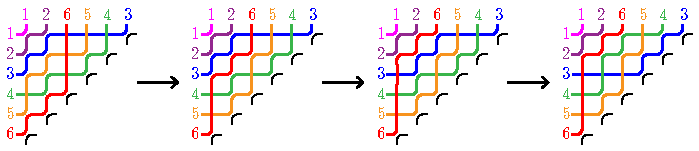
\includegraphics[scale=1.3]{counterExampleRestrictionIncreasingFlipPoset}}
	\caption{Two acyclic pipe dreams~$\acyclicPipeDreams(126543)$ connected by a sequence of increasing flips in~$\pipeDreams(126543)$ but by no sequence of increasing flips in~$\acyclicPipeDreams(126543)$.}
	\label{fig:counterExampleRestrictionIncreasingFlipPoset}
\end{figure}
\end{remark}

To prove \cref{thm:pipeDreamQuotient}, we need the following auxiliary statement.

\begin{lemma}
\label{lem:flippable}
Consider two acyclic pipe dreams~$P,P' \in \acyclicPipeDreams(\omega)$ connected by the flip of a contact between their pipes~$i$ and~$j$.
Then any directed path in~$P\contact$ or~$P'{}\contact$ between~$i$ and~$j$ is an arc.
\end{lemma}

\begin{proof}
Say that~$i < j$ while~$\omega^{-1}(i) > \omega^{-1}(j)$ and that~$i \to j$ is an arc of~$P\contact$ while~$j \to i$ is an arc of~$P'{}\contact$.
Since $P\contact$ is acyclic, there is no path from~$j$ to~$i$ in~$P\contact$.
Assume by means of contradiction that there is a path~$i \to k_1 \to \dots \to k_p \to j$ in~$P\contact$ with~$p \ge 1$.
Since the arcs of~$P'{}\contact$ are the arcs of~$P\contact$ where only extremities~$i$ and~$j$ can be changed, $P'{}\contact$ contains the path~$k_1 \to \dots \to k_p$ and at least one of the arcs~$i \to k_1$ or~$j \to k_1$, and at least one of the arcs~$k_p \to j$ or~$k_p \to i$.
Consequently, since~$P'{}\contact$ contains the arc~$j \to i$ and is acyclic, it must contain the path~$j \to k_1 \to \dots \to k_p \to i$.
We thus obtained that~$i \contactLess{P} k_1 \contactLess{P} j$ while~$i \contactMore{P'} k_1 \contactMore{P'} j$, and~$k_1$ has a contact with~$i$ in~$P$ that becomes a contact with~$j$ in~$P'$.

Consider now the contact~$c$ of~$P$ which is a crossing in~$P'$ and the contact~$c'$ of~$P'$ which is a crossing of~$P$.
Let~$R$ the rectangle with corners~$c$ and~$c'$.
Since~$k_1$ has a contact with~$i$ in~$P$ and with~$j$ in~$P'$, it must pass inside~$R$.
Since~$i \contactLess{P} k_1 \contactLess{P} j$ and~$i \contactMore{P'} k_1 \contactMore{P'} j$, the pipe~$k$ has no elbow located northwest or southeast of~$c$ or~$c'$, hence no elbow located north, south, west or east of~$R$.
We thus obtain that~$k$ must be straight before it reaches~$R$, and after it leaves~$R$.
Hence $k_1 < i < j$ and~$\omega^{-1}(k_1) > \omega^{-1}(j) > \omega^{-1}(i)$.
By \cref{lem:consequenceRectangle1}, this contradicts~$i \contactLess{P} k_1$~and~$k_1 \contactMore{P'} j$.
\end{proof}

\begin{proof}[Proof of \cref{thm:pipeDreamQuotient}]
We need to prove that the following conditions are equivalent for two distinct pipe dreams~$P,P' \in \acyclicPipeDreams(\omega)$:
\begin{enumerate}[(i)]
\item there is an increasing flip from $P$ to~$P'$,
\item there exist linear extensions~$\pi$ of~$P$ and~$\pi'$ of~$P'$ such that~$\pi'$ covers~$\pi$ in weak order.
\end{enumerate}
\cref{lem:lowerSetPipeDreams,thm:partitionPipeDreams} directly imply that (ii) $\Rightarrow$ (i).
For (i) $\Rightarrow$ (ii), let~$i < j$ be the two pipes involved in the flip between~$P$ and~$P'$.
Hence, $i \to j$ is an arc of~$P\contact$ while~$j \to i$ is an arc of~$P'{}\contact$.
By \cref{lem:flippable}, there is no directed path from~$i$ to~$j$ in~$P\contact$ besides the arcs~$i \to j$ (there might be more than one such arc).
Hence, there exists a linear extension~$\pi$ of~$P$ where~$i$ and~$j$ are consecutive.
Write~$\pi \eqdef UijV$ and define~$\pi' \eqdef UjiV$.
Since~$i \to j$ is an arc of~$P\contact$, $\pi'$ is not a linear extension of~$P$.
Hence, by \cref{lem:lowerSetPipeDreams}, $\pi'$ is a linear extension of~$P'$.
\end{proof}

Let us conclude by providing more equivalent characterizations of the increasing flip lattice lattice on~$\acyclicPipeDreams(\omega)$.

\begin{proposition}
For any pipe dreams~$P, P' \in \acyclicPipeDreams(\omega)$, the following assertions are equivalent:
\begin{enumerate}[(i)]
\item there is a path from $P$ to~$P'$ in the increasing flip graph on~$\acyclicPipeDreams(\omega)$,
\item there exist linear extensions~$\pi$ of~$P$ and~$\pi'$ of~$P'$ such that~$\pi < \pi'$ in weak order,
\item the minimal (resp.~max) linear extensions~$\pi$ of~$P$ and~$\pi'$ of~$P$ satisfy~$\pi < \pi'$ in weak order.
\item there is no~$i < j$ such that~$i \contactMore{P} j$ and~$i \contactLess{P'} j$,
\item for all~$i < j$, if~$i \contactMore{P} j$, then~$j \contactMore{P'} i$,
\item for all~$i < j$, if~$i \contactLess{P'} j$, then~$i \contactLess{P} j$,
\end{enumerate}
\end{proposition}

\begin{proof}
We already proved the equivalence (i) $\Leftrightarrow$ (ii) in \cref{thm:pipeDreamQuotient}.
The equivalence (ii) $\Leftrightarrow$ (iii) is valid for any lattice quotient.
The equivalences (iii) $\Leftrightarrow$ (iv) $\Leftrightarrow$ (v) $\Leftrightarrow$ (vi) follow from the descriptions of \cref{prop:WOIP} for the inversions of the minimum and the non-inversions of the maximum of a weak order interval.
\end{proof}

%%%%%%%%%%%%%%%%%%%%%%%%%%%%%%%%%%%%%%
%%%%%%%%%%%%%%%%%%%%%%%%%%%%%%%%%%%%%%
%%%%%%%%%%%%%%%%%%%%%%%%%%%%%%%%%%%%%%

\section{Further topics on pipe dreams}
\label{sec:furtherTopics}

In this section, we discuss four further topics on the pipe dream congruence.
We first describe two algorithms to construct the pipe dream~$\insertion{\pi}{\omega}$ of~$\acyclicPipeDreams(\omega)$ of which a given permutation~$\pi$ is a linear extension (\cref{subsec:sweepingAlgorithm,subsec:insertionAlgorithm}).
We then describe the pipe dream congruence~$\equiv_\omega$ as the transitive closure of a rewriting rule on permutations of~$[e, \omega]$ (\cref{subsec:rewritingRule}).
Finally, we describe the natural coarsening of the pipe dream congruence~$\equiv_\omega$ by the recoil congruence~$\cong_\omega$ (\cref{subsec:canopy}).

%To sum up, there are three equivalent ways to partition the interval~$[e,\omega]$ of the weak order:
%\begin{itemize}
%\item by the sets of linear extensions~$\linearExtensions(P)$ of all pipe dreams of~$\acyclicPipeDreams(\omega)$,
%\item by the fibers of the sweeping algorithm, \vincent{choose notation}
%\item by the fibers of the insertion map~$\insertion{\cdot}{\omega}$,
%\item by the classes of the pipe dream congruence~$\equiv_\omega$.
%\end{itemize}

%%%%%%%%%%%%%%%%%%%%%%%%%%%%%%%%%%%%%%

\subsection{Sweeping algorithm}
\label{subsec:sweepingAlgorithm}

Our first algorithm to construct~$\insertion{\pi}{\omega}$ is a \defn{sweeping algorithm}, inspired by the algorithm to compute greedy pipe dreams~\cite{PilaudPocchiola, PilaudStump-ELlabelings}.
An extension of this algorithm to subword complexes will be discussed in \cref{subsec:sweepingAlgorithmSubwordComplexes}, and appeared independently in~\cite{JahnStump}.

\begin{proposition}
\label{prop:sweepingAlgorithm}
For any permutations~$\pi,\omega \in \fS_n$ such that~$\pi < \omega$ in weak order, the unique pipe dream~$P \in \acyclicPipeDreams(\omega)$ such that~$\pi \in \linearExtensions(P)$ can be constructed by sweeping the triangular shape in any perturbation of the northwest direction and placing a crossing when sweeping a vertex~$v$ of the grid where pipe~$i$ arrives horizontally and pipe~$j$ arrives vertically if and only if
\begin{itemize}
\item $i < j$ and~$\omega^{-1}(i) > \omega^{-1}(j)$, and 
\item $\pi^{-1}(i) > \pi^{-1}(j)$ or vertex~$v$ lies in column~$\omega^{-1}(j)$.
\end{itemize}
See \cref{fig:sweepingAlgorithm}.
\end{proposition}

\begin{example}
\label{exm:sweepingAlgorithm}
\cref{fig:sweepingAlgorithm} illustrates the sweeping algorithm for the permutations~${\pi = 513264}$ and~${\omega = 561324}$.
The algorithm has 15 steps, but we have grouped together steps $2$ to $9$ (second arrow) and steps $12$ to $13$ (fifth arrow) as they have the same justification.
We place contacts in steps $1$, $10$, $12$, $13$ and~$15$ since~$\omega^{-1}(i) < \omega^{-1}(j)$, and in step~$14$ since~$i > j$.
We place crossings in steps $2$ to $9$ since~$i < j$, $\omega^{-1}(i) > \omega^{-1}(j)$ and we are in the column~$\omega^{-1}(j)$, and in step $11$ since~$i < j$, $\omega^{-1}(i) > \omega^{-1}(j)$ and~$\pi^{-1}(i) > \pi^{-1}(j)$.
%
\begin{figure}[b]
	\centerline{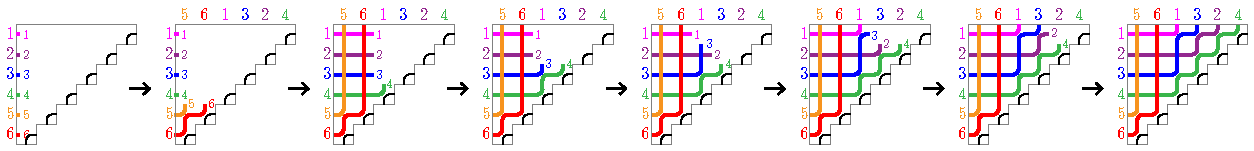
\includegraphics[scale=.9]{sweeping}}
	\caption{Sweeping algorithm for the permutations~$\pi = 513264$ and~$\omega = 561324$.} % See details in \cref{exm:sweepingAlgorithm}.}
	\label{fig:sweepingAlgorithm}
\end{figure}
\end{example}

\begin{proof}[Proof of \cref{prop:sweepingAlgorithm}]
When we sweep vertex~$v$ where pipe~$i$ arrives horizontally and pipe~$j$ arrives vertically,
\begin{itemize}
\item we have no choice but imposing a contact at~$v$ if~$i > j$ (since pipes $i$ and~$j$ already crossed before) or~$\omega^{-1}(i) < \omega^{-1}(j)$ (since pipes~$i$ and~$j$ do not cross at all),
\item if~$i < j$ and~$\omega^{-1}(i) > \omega^{-1}(j)$, then
\begin{itemize}
\item if~$\pi^{-1}(i) > \pi^{-1}(j)$ then pipes~$i$ and~$j$ cannot touch (otherwise $\pi$ would not be a linear extension of~$P$), so that we have no choice but imposing a crossing~at~$v$,
\item if~$\pi^{-1}(p) < \pi^{-1}(q)$ then
	\begin{itemize}
	\item if $v$ lies in column~$\omega^{-1}(j)$, then pipe $j$ needs to go straight north, and we have no choice but imposing a crossing at~$v$,
	\item otherwise, we have no choice but imposing a contact at~$v$ (otherwise \cref{lem:rectangle} ensures that~$j \contactLess{P} i$, so that~$\pi$ would not be a linear extension of~$P$).
	\qedhere
	\end{itemize}
\end{itemize}
\end{itemize}
\end{proof}

%%%%%%%%%%%%%%%%%%%%%%%%%%%%%%%%%%%%%%

\subsection{Insertion algorithm}
\label{subsec:insertionAlgorithm}

Our second algorithm to construct~$\insertion{\pi}{\omega}$ is an \defn{insertion algorithm} inspired from~\cite{Pilaud-brickAlgebra} and similar to the insertion in binary search trees.

We call \defn{staircase} of length~$k$ a sequence~$e_1, \dots, e_k$ of southeast elbows such that~$e_i$ is located strictly southwest of~$e_{i+1}$ for each~$i \in [k-1]$. In other words, $r_1 > \dots > r_k$ and~$c_1 < \dots < c_k$ where~$e_i$ is located in row~$r_i$ and column~$c_i$.
For~$j \in [n]$ such that~$j > r_1$ and~$c_k < \omega^{-1}(j)$, there is a unique pipe which enters at row~$j$, exits at column~$\omega^{-1}(j)$, and whose northeast elbows are precisely covering the southeast elbows~$e_1, \dots, e_k$.
Namely, it has a northeast elbow at row~$r_i$ and column~$c_i$ for each~$i \in [k]$, and a southeast elbow at row~$r_{i-1}$ and column~$c_i$ for each~$i \in [k+1]$, where by convention~$r_0 \eqdef j$ and~$c_{k+1} \eqdef \omega^{-1}(j)$.

\begin{proposition}
\label{prop:insertionAlgorithm}
For any permutations~$\pi,\omega \in \fS_n$ such that~$\pi < \omega$ in weak order, the unique pipe dream~$P \in \acyclicPipeDreams(\omega)$ such that~$\pi \in \linearExtensions(P)$ can be constructed starting from the empty triangular shape and inserting the pipes~$\pi(1), \dots, \pi(n)$ one by one in the order of the permutation~$\pi$ as northwest as possible.
More precisely, at step~$t$, we insert a pipe starting at row~$\pi(t)$, ending at column~$\omega^{-1}(\pi(t))$, and whose northeast elbows are precisely covering the staircase of currently free southeast elbows in the rectangle~$[\pi(t)] \times [\omega^{-1}(\pi(t))]$.
%More precisely, at step~$t$, we consider the set~$X_t$ of free southeast elbows in the rectangle~$[\pi(t)] \times [\omega^{-1}(\pi(t))]$, and we insert a pipe starting at row~$\pi(t)$, ending at column~$\omega^{-1}(\pi(t))$, and whose northeast elbows are precisely covering the elbows of~$X_t$, and adding a new free southeast elbow in between any two consecutive elbows of~$X_t$
See \cref{fig:insertionAlgorithm}.
\end{proposition}

\begin{example}
\label{exm:insertionAlgorithm}
\cref{fig:insertionAlgorithm} illustrates the insertion algorithm for the permutations~${\pi = 513264}$ and~${\omega = 561324}$.
For instance, when inserting the (green) pipe~$4$ in the last step, the currently free southeast elbows are the first southeast elbow of the (blue) pipe~$3$ and the two southeast elbows of the (purple) pipe~$2$.
%
\begin{figure}[b]
	\centerline{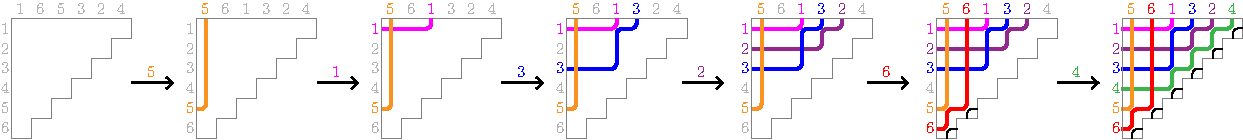
\includegraphics[scale=.9]{insertion}}
	\caption{Insertion algorithm for the permutations~$\pi = 513264$ and~$\omega = 561324$.}
	\label{fig:insertionAlgorithm}
\end{figure}
\end{example}

We need to argue that this algorithm indeed creates a pipe dream of~$\pipeDreams(\omega)$.
To see it, we observe that the following two invariants are maintained throughout the algorithm.
We call \defn{hook} of a southeast elbow~$e$ the union of the horizontal segment west of~$e$ and the vertical segment north of~$e$.

\begin{lemma}
\label{lem:disjointPipesInsertionAlgorithm}
At any time during the insertion algorithm, the support of the pipes already inserted is precisely the union of the hooks of the currently free southeast elbows.
\end{lemma}

\begin{proof}
Immediate by induction, as the support of a pipe is precisely the union of the hooks of its southeast elbows minus the union of the pipes of its northeast elbows.
\end{proof}

\begin{corollary}
\label{coro:disjointPipesInsertionAlgorithm}
The pipes constructed by the insertion algorithm are disjoint, except at crossings and contacts.
\end{corollary}

\begin{lemma}
\label{lem:rectangleInsertionAlgorithm}
For any~$t, r, c \in [n]$, the free southeast elbows in the rectangle~$[r] \times [c]$ just before step~$t$ of the insertion algorithm form a staircase of length
\[
\# \set{s < t}{\pi(s) \le r \text{ and } \omega^{-1}(\pi(s)) \le c} - \# \set{s < t}{\pi(s) > r \text{ and } \omega^{-1}(\pi(s)) > c}.
\]
\end{lemma}

\begin{proof}
Denote by~$R$ the rectangle~$[r] \times [c]$.
The proof works by induction on~$t$.
Before step~$1$, there is no southeast elbow in~$R$.
Assume now that just before step~$t$, the free southeast elbows in~$R$ form a staircase~$e_1, \dots, e_k$ with~$k$ given by the formula of the statement.
At step~$t$, we insert a new pipe~$\pi(t)$ which enters at~$\pi(t)$ and exits at~$\omega^{-1}(\pi(t))$.
Let~${0 \le i < j \le k+1}$ be such that~$e_{i+1}, \dots, e_{j-1}$ are the northwest elbows of pipe~$\pi(t)$ in~$R$, and let~$e'_1, \dots, e'_\ell$ be the southeast elbows of pipe~$\pi(t)$ in~$R$.
Hence, the free southeast elbows in~$R$ after step~$t$ form the sequence~$e_1, \dots, e_i, e'_1, \dots, e'_\ell, e_j, \dots, e_k$.
We thus just need to see that $e_i$ is southwest of~$e'_1$ and~$e'_\ell$ is southwest of~$e_j$, and that
\[
\ell = \begin{cases} j-i  & \text{if } \pi(s) \le r \text{ and } \omega^{-1}(\pi(s)) \le c, \\  j-i-2  & \text{if } \pi(s) > r \text{ and } \omega^{-1}(\pi(s)) > c, \\  j-i-1 & \text{otherwise.} \end{cases}
\]
Since the northwest and southeast elbows alternate along pipe~$\pi(t)$, this follows from the fact that the pipe~$\pi(t)$ enters~$R$ with an horizontal step if~$\pi(t) \le r$ and with a vertical step if~$\pi(s) > r$, and exits~$R$ with a vertical step if~$\omega^{-1}(\pi(t)) \le c$ and with an horizontal step if~$\omega^{-1}(\pi(s)) > c$.
%setting~$i \eqdef \pi(t)$ and~$j \eqdef \pi(s)$, we have~${i < j}$ and~$\pi^{-1}(i) > \pi^{-1}(j)$ while~$\omega^{-1}(i) < \omega^{-1}(j)$, which contradicts our assumption that~$\pi < \omega$. \qedhere
\end{proof}

We now derive two properties of the insertion algorithm from \cref{lem:rectangleInsertionAlgorithm}.
Recall that we denote by~$\noninversions{\omega}{j} \eqdef \#\set{i \in [n]}{i < j \text{ and } \omega^{-1}(i) < \omega^{-1}(j)}$ the number of non-inversions of~$j$ in a permutation~$\omega$.

\begin{corollary}
\label{coro:rectangleInsertionAlgorithm1}
For any~$t \in [n]$, the free southeast elbows in the rectangle~$[\pi(t)] \times [\omega^{-1}(\pi(t))]$ just before step~$t$ of the insertion algorithm form a staircase of length~$\noninversions{\omega}{\pi(t)}$.
\end{corollary}

\begin{proof}
Observe first that if there if~$r < s$ such that~$\pi(r) > \pi(s)$ and~$\omega^{-1}(\pi(r)) > \omega^{-1}(\pi(s))$, then setting~$i \eqdef \pi(s)$ and~$j \eqdef \pi(r)$, we have~${i < j}$ and~$\pi^{-1}(i) > \pi^{-1}(j)$ while~$\omega^{-1}(i) < \omega^{-1}(j)$, which contradicts our assumption that~$\pi < \omega$.
This implies that
\begin{align*}
\# \set{s < t}{\pi(s) < \pi(t) \text{ and } \omega^{-1}(\pi(s)) < \omega^{-1}(\pi(t))} & = \noninversions{\omega}{\pi(t)} \\
\text{and}\qquad \# \set{s < t}{\pi(s) > \pi(t) \text{ and } \omega^{-1}(\pi(s)) > \omega^{-1}(\pi(t))} & = 0.
\end{align*}
Hence, the result follows from~\cref{lem:rectangleInsertionAlgorithm} applied to the parameters~$t, \pi(t), \omega^{-1}(\pi(t))$.
\end{proof}

\begin{corollary}
\label{coro:rectangleInsertionAlgorithm2}
All pipes of constructed by the insertion algorithm remain in the triangular shape.
\end{corollary}

\begin{proof}
Let~$1 \le i \le j \le n$.
Note that
\[
j - \noninversions{\omega}{j} = \#\set{i \in [n]}{i < j \text{ and } \omega^{-1}(i) > \omega^{-1}(j)} + 1 \le n - \omega^{-1}(j) + 1,
\]
so that~$\omega^{-1}(j) - \noninversions{\omega}{j} + j \ge n + 1$.
By~\cref{lem:rectangleInsertionAlgorithm}, the pipe~$j$ has~$\noninversions{\omega}{j}$ southeast elbows in total, at most~$j-i-1$ of which are strictly south of row~$i$, so that at least~$\noninversions{\omega}{j} - j + i$ of which are strictly north of row~$i$.
Hence, the eastmost point of pipe~$j$ in row~$i$ is at most in column~$\omega^{-1}(j) - \noninversions{\omega}{j} + j - i \le n - i + 1$.
We conclude that pipe~$j$ indeed remains in the triangular shape.
\end{proof}

\begin{proof}[Proof of \cref{prop:insertionAlgorithm}]
The insertion algorithm constructs a collection~$P$ of $n$ pipes in the triangular shape (by \cref{coro:rectangleInsertionAlgorithm2}), which are pairwise disjoint except at crossings and contacts (by \cref{coro:disjointPipesInsertionAlgorithm}).
For each~$t \in [n]$, the pipe~$\pi(t)$ enters at row~$\pi(t)$, exits at column~$\omega^{-1}(\pi(t))$, and has~$\noninversions{\omega}{\pi(t)}$ many southeast contacts (by \cref{coro:rectangleInsertionAlgorithm1}).
We thus conclude that~$P$ is a pipe dream of~$\pipeDreams(\omega)$ by a direct application of \cref{lem:characterizationPipeDreams}.

By construction, all southeast contacts of the pipe~$\pi(t)$ inserted at step~$t$ are in contact with northwest contacts of pipes~$\pi(s)$ inserted at steps~$s < t$.
In other words, all edges in the contact graph of~$\insertion{\pi}{\omega}$ are of the form~$\pi(s) \to \pi(t)$ for some~$s < t$.
It follows that the permutation~$\pi$ is a linear extension of the pipe dream~$P$.
\end{proof}

%%%%%%%%%%%%%%%%%%%%%%%%%%%%%%%%%%%%%%

\subsection{Rewriting rule}
\label{subsec:rewritingRule}

Recall from \cref{exm:Tamari3} that the sylvester congruence can be defined as the transitive closure of the classical rewriting rule~$UjVikW \equiv UjVkiW$ where~$i < j < k$ are elements of~$[n]$ while~$U, V, W$ are (possibly empty) words on~$[n]$ (as usual, we write the permutations of~$\fS_n$ as words in one-line notation).
We now describe a similar rewriting rule for the pipe dream congruence~$\equiv_\omega$.

\begin{proposition}
\label{prop:rewritingRule}
On the interval~$[e,\omega]$ of the weak order, the pipe dream congruence~$\equiv_\omega$ coincides with the transitive closure of the rewriting rule~$U ij V \equiv_\omega U ji V$ where~$1 \le i < j \le n$ are elements of~$[n]$ while~$U, V$ are (possibly empty) words on~$[n]$ such that
\[
\# \set{k \in U}{k > i} \ge \# \set{k \in U}{\omega^{-1}(k) < \omega^{-1}(j)}.
\]
\end{proposition}

\begin{proof}
As they are linear extensions of posets, the congruence classes of $\equiv_\omega$ are connected by simple transpositions.
We thus just need to show that any two permutations~$\pi \eqdef UijV$ and~$\pi' \eqdef UjiV$ of~$[e, \omega]$ which differ by the inversion of two consecutive values are equivalent for~$\equiv_\omega$ if and only if~$\# \set{k \in U}{k > i} \ge \# \set{k \in U}{\omega^{-1}(k) < \omega^{-1}(j)}$.
Moreover, by \cref{prop:insertionAlgorithm}, $\pi \equiv_\omega \pi'$ if and only if they are sent to the same pipe dream by the insertion algorithm.
Let~$t \eqdef \pi^{-1}(i) = \pi'^{-1}(j)$.
Before step~$t$ of the insertion algorithm, we insert the word~$U$ both for~$\pi$ and for~$\pi'$.
The insertion of~$i$ and~$j$ then commute if and only if there is no currently free elbow in the rectangle~$[i] \times [\omega^{-1}(j)]$.
By \cref{lem:rectangleInsertionAlgorithm} applied to the parameters~$t, i, \omega^{-1}(j)$, this is equivalent to
\[
\# \set{s < t}{\pi(s) \le i \text{ and } \omega^{-1}(\pi(s)) \le \omega^{-1}(j)} \le \# \set{s < t}{\pi(s) > i \text{ and } \omega^{-1}(\pi(s)) > \omega^{-1}(j)}.
\]
or written differently,
\[
\# \set{k \in U}{k < i \text{ and } \omega^{-1}(k) < \omega^{-1}(j)} \le \# \set{k \in U}{k > i \text{ and } \omega^{-1}(k) > \omega^{-1}(j)}.
\]
(note that  to replace large by strict inequalities in the first set, we used that~$k \ne i$ and ${\omega^{-1}(k) \ne \omega^{-1}(j)}$ since~$i,j \notin U$ while~$k \in U$).
Finally, observe that adding~$\# \set{k \in U}{k > i \text{ and } \omega^{-1}(k) < \omega^{-1}(j)}$ from both side, we obtain the equivalent condition
\[
\# \set{k \in U}{\omega^{-1}(k) < \omega^{-1}(j)} \le \# \set{k \in U}{k > i}.
\qedhere
\]
\end{proof}

\begin{remark}
\label{rem:rewritingRule}
Observe from the proof that the condition of \cref{prop:rewritingRule} is equivalent to
\[
\# \set{k \in U}{k < i \text{ and } \omega^{-1}(k) < \omega^{-1}(j)} \le \# \set{k \in U}{k > i \text{ and } \omega^{-1}(k) > \omega^{-1}(j)}.
\]
Observe moreover that since~$\pi \le \omega$ and~$i < j$, we have
\begin{align*}
\set{k \in U}{k < i \text{ and } \omega^{-1}(k) < \omega^{-1}(j)} & = \set{k \in [i]}{\omega^{-1}(k) < \omega^{-1}(j)} \qquad \text{and}\\
\set{k \in U}{k > i \text{ and } \omega^{-1}(k) > \omega^{-1}(j)} & = \set{k \in [n]}{i < k < j \text{ and } \omega^{-1}(i) > \omega^{-1}(k) > \omega^{-1}(j)}.
\end{align*}
\end{remark}

We close this section by two immediate consequences of \cref{prop:rewritingRule,rem:rewritingRule}.

\begin{corollary}
\label{coro:patternAvoiding}
A permutation is minimal (resp.~maximal) in its pipe dream congruence class if and only if it avoids the patters~$k_1 - \cdots - k_p - ji$ (resp.~$k_1 - \cdots - k_p - ij$) where~$k_q > i$ and~$\omega^{-1}(k_q) > \omega^{-1}(j)$ for~$q \in [p]$ and~$p = \# \set{k \in [i]}{\omega^{-1}(k) < \omega^{-1}(j)}$.
\end{corollary}

\begin{proof}
This is an immediate consequence of \cref{prop:rewritingRule}: a permutation~$\pi$ is minimal (resp.~maximal) in its $\equiv_\omega$-congruence class if and only if it contains no consecutive exchangeable entries~$ji$ (resp.~$ij$) with~$i < j$.
\end{proof}

\begin{corollary}
\label{coro:canopy}
If~$1 \le i < j \le n$ and~$j-i \le \#\set{k \in [i]}{\omega^{-1}(k) < \omega^{-1}(j)}$, then the pipes~$i$ and~$j$ are comparable for $\contactLess{P}$ in any acyclic pipe dream~$P \in \acyclicPipeDreams(\omega)$.
\end{corollary}

\begin{proof}
If pipes~$i$ and~$j$ were incomparable in~$\contactLess{P}$, there would be two permutations~$UijV \equiv_\omega UjiV$.
However, $j-i \le \#\set{k \in [i]}{\omega^{-1}(k) < \omega^{-1}(j)}$ implies that the condition of \cref{prop:rewritingRule} cannot hold, by \cref{rem:rewritingRule}
\end{proof}


%%%%%%%%%%%%%%%%%%%%%%%%%%%%%%%%%%%%%%

\subsection{Recoils and canopy}
\label{subsec:canopy}

To conclude, we generalize the notion of recoils of permutations and of canopy of a binary trees to show a natural commutative diagram of lattice homomorphisms.
We start with the easy generalization of recoils of a permutation.

\begin{definition}
\label{def:recoils}
Consider the graph~$G(\omega)$ with vertex set~$[n]$ and edge set
\[
\set{ik}{i < j \text{ and } j-i \le \#\set{k \in [i]}{\omega^{-1}(k) < \omega^{-1}(j)}}.
\]
Let~$\acyclicOrientations(\omega)$ denote the set of acyclic orientations of~$G(\omega)$.
The \defn{$\omega$-recoil congruence} is the equivalence relation on the weak order interval~$[e, \omega]$ whose equivalence classes are the sets of linear extensions of the acyclic orientations of~$G(\omega)$.
The \defn{$\omega$-recoils} of a permutation~$\pi \in [e,\omega]$ is the acyclic orientation~${\recoils{\pi}{\omega} \in \acyclicOrientations(\omega)}$ such that~$\pi$ is a linear extension of~$\recoils{\pi}{\omega}$.
\end{definition}

We now generalize the canopy of a binary tree.
Recall that the \defn{canopy} of a binary tree~$T$ with~$n$ internal nodes is the sign sequence~${\canopy{T} \in \{{-},{+}\}^{n-1}}$ defined by~$\canopy{T}_i = {-}$ if the $(i+1)$st leaf of~$T$ is a left leaf and~$\canopy{T}_i = {+}$ if the $(i+1)$st leaf of~$T$ is a right leaf.
Equivalently, $\canopy{T}_i = -$ if the node~$i$ of~$T$ is above the node~$i+1$ of~$T$ and~$\canopy{T}_i = +$ otherwise.
This map was already used by J.-L.~Loday in~\cite{LodayRonco, Loday}, but the name ``canopy'' was coined by X.~Viennot~\cite{Viennot}.
We now define a generalization of the canopy map for pipe dreams in~$\acyclicPipeDreams(\omega)$, using \cref{coro:canopy}.

\begin{definition}
\label{def:canopy}
The \defn{canopy} of a pipe dream~$P \in \acyclicPipeDreams(\omega)$ is the orientation~$\canopy{P} \in \acyclicOrientations(\omega)$ where each edge~$ij$ is oriented~$i \to j$ if~$i \contactLess{P} j$ and~$j \to i$ if~$j \contactLess{P} i$.
\end{definition}

\begin{proposition}
\label{prop:latticeHomomorphisms}
The maps~$\recoils{\cdot}{\omega}$, $\insertion{\cdot}{\omega}$, and~$\canopy{\cdot}$ define the following commutative diagram of lattice homomorphisms:
\[
\begin{tikzpicture}
  \matrix (m) [matrix of math nodes,row sep=1.2em,column sep=5em,minimum width=2em]
  {
     [e,\omega]  	&								& \acyclicOrientations(\omega)	\\
					& \acyclicPipeDreams(\omega) 	&								\\
  };
  \path[->] (m-1-1) edge node [above] {$\recoils{\cdot}{\omega}$} (m-1-3);
  \path[->>] (m-1-1) edge node [below] {$\insertion{\cdot}{\omega}\qquad$} (m-2-2.west);
  \path[->] (m-2-2.east) edge node [below] {$\quad\canopy{\cdot}$} (m-1-3);
\end{tikzpicture}
\]
\end{proposition}

\begin{proof}
Consider a permutation~$\pi$ and let~$i < j \in [n]$ be such that~$j-i \le \#\set{k < i}{\omega^{-1}(k) < \omega^{-1}(j)}$.
Assume that the edge~$ij$ is oriented from~$i$ to~$j$.
Then~$\pi^{-1}(i) < \pi^{-1}(j)$, thus the pipe~$i$ is inserted before the pipe~$j$ in~$\insertion{\pi}{\omega}$, so that~$i \contactLess{\insertion{\pi}{\omega}} j$ and there is also an arc from~$i$ to~$j$ in~$\canopy{\insertion{\pi}{\omega}}$.
\end{proof}

%%%%%%%%%%%%%%%%%%%%%%%%%%%%%%%%%%%%%%
%%%%%%%%%%%%%%%%%%%%%%%%%%%%%%%%%%%%%%
%%%%%%%%%%%%%%%%%%%%%%%%%%%%%%%%%%%%%%

\section{Subword complexes}
\label{sec:subwordComplexes}

The objective of this section is to partially extend our results about the lattice structure of acyclic pipe dreams (\cref{sec:latticeAcyclicPipeDreams}) to the wider context of subword complexes in finite Coxeter groups.
We start with some basic preliminaries on finite Coxeter groups (\cref{subsec:finiteCoxeterGroups}) and subword complexes (\cref{subsec:subwordComplexes}).
We then define linear extensions of facets of subword complexes (\cref{subsec:linearExtensionsFacets}) and present two theorems (\cref{subsec:twoTheorems}) and five conjectures (\cref{subsec:fiveConjectures}) about them.
To conclude, we present a sweeping algorithm to construct the facet with a given linear extension (\cref{subsec:sweepingAlgorithmSubwordComplexes})

%%%%%%%%%%%%%%%%%%%%%%%%%%%%%%%%%%%%%%

\subsection{Finite coxeter groups} 
\label{subsec:finiteCoxeterGroups}

We refer to~\cite{BjornerBrenti, Humphreys} for detailed references on Coxeter groups. 
We consider a \defn{finite root system} $\Phi$ with \defn{positive roots}~$\Phi^+$, \defn{negative roots}~$\Phi^+-$, and \defn{simple roots} $\Delta \subseteq \Phi^+$.
The reflections along the hyperplanes orthogonal to the roots in $\Phi$ generate a \defn{finite Coxeter group} $W$.
We denote by~$s_\alpha \in W$ the reflection orthogonal to a root~$\alpha \in \Phi$, and by~$\alpha_s \in \Phi^+$ the positive root orthogonal to a reflection~$s \in W$.
The group~$W$ is actually generated by the simple reflections~$S = \set{s_\alpha}{\alpha \in \Delta}$, and the pair~$(W,S)$ is a \defn{finite Coxeter system}.
Finite root systems and finite Coxeter systems are classified in terms of Dynkin diagrams, see~\cite{Humphreys}. 

The \defn{inversion set}~$\Inv(\omega)$ and the \defn{non-inversion set}~$\Ninv(\omega)$ of an element~$\omega \in W$ are
\[
\Inv(\omega) \eqdef \Phi^+ \cap \omega(\Phi^-)
\qquad\text{and}\qquad
\Ninv(\omega) \eqdef \Phi^+ \cap \omega(\Phi^+).
\]
Note that
\[
\Phi^+ = \Inv(\omega) \sqcup \Ninv(\omega)
\qquad\text{and}\qquad
\omega(\Phi^+) = -\Inv(\omega) \sqcup \Ninv(\omega).
\]

A \defn{reduced expression} of~$\omega$ is a product~$s_1 s_2 \dots s_\ell = \omega$ of simple reflections~$s_i \in S$ such that~$\ell$ is minimal.
This minimal~$\ell$ is the \defn{length} $\ell(\omega)$ of~$\omega$.
The length of~$\omega$ coincides with the size of its inversion set~$\Inv(\omega)$ since $\Inv(\omega) \eqdef \{\alpha_{s_1}, s_1(\alpha_{s_2}), s_1s_2(\alpha_{s_3}), \dots, s_1s_2 \dots s_{\ell-1}(\alpha_{s_\ell})\}$.

The \defn{weak order} on $W$ is the partial order $\le$ defined by $\sigma \leq \omega$ if there exists $\tau \in W$ such that $\sigma\tau = \omega$ and $\ell(\sigma) + \ell(\tau) = \ell(\omega)$.
In other words, the element $\omega$ has a reduced expression with a prefix which is a reduced expression of $\sigma$.
Equivalently, the weak order corresponds to the inclusion order on inversion sets, that is $\sigma \leq \omega$ if and only if $\Inv(\sigma) \subseteq \Inv(\omega)$.
This order defines a lattice structure on the elements of~$W$.
The minimal element is the identity $e \in W$ and the maximal element is the \defn{unique longest element} $\wo$ of~$W$.
Note that~$\Inv(e) = \varnothing = \Ninv(\wo)$ and~$\Ninv(e) = \Phi^+ = \Inv(\wo)$, so that~$\ell(e) = 0$ while~$\ell(\wo) = |\Phi^+|$.
% Note also that~$\Ninv(\omega) =\Inv(\omega\wo)$.

\begin{example}
\label{exm:typeACoxeterSystem}
The Coxeter system of type~$A_{n-1}$ is the symmetric group~$W = \fS_n$ with generators~$S = \set{\tau_i}{i \in [n-1]}$, where~$\tau_i$ is the simple transposition~$\tau_i = (i \; i+1)$.
It naturally acts on~$\R^n$ by permutations of coordinates.
Denoting by~$(\b{e}_i)_{i \in [n]}$ the canonical basis of~$\R^n$, the type~$A_{n-1}$ roots are all~$\b{r}_{i,j} \eqdef \b{e}_i - \b{e}_j$ for distinct~$i,j \in [n]$, with positive roots~$\b{r}_{i,j}$ for~$1 \le i < j \le n$ and simple roots~$\b{r}_{i,i+1}$ for~$i \in [n-1]$.
The inversion set of~$\pi \in \fS_n$ is the set of roots~$\b{e}_i - \b{e}_j$ for the inversions~$(i,j)$ of the permutation~$\pi$.
The longest element is the reversed permutation~$[n, n-1, \dots, 2, 1]$ (written in one line notation), and it admits the reduced expression~$\tau_1 \cdots \tau_{n-1} \tau_1 \cdots \tau_{n-2} \cdots \tau_1 \tau_2 \tau_1$.
\end{example}

%%%%%%%%%%%%%%%%%%%%%%%%%%%%%%%%%%%%%%

\subsection{Subword complexes}
\label{subsec:subwordComplexes}

Motivated by their study of Gröbner geometry of Schubert varieties~\cite{KnutsonMiller-GroebnerGeometry}, A.~Knutson and E.~Miller introduced in~\cite{KnutsonMiller-subwordComplex} the following remarkable family of simplicial complexes in the context of Coxeter groups.

Let $(W,S)$ be a finite Coxeter system, $Q=(q_1,\dots,q_m)$ be a word in the simple reflections $S$, and $\omega \in W$ be an element of the group.
For $J\subseteq [r]$, we denote by $Q_J$ the subword of~$Q$ consisting of the letters with positions in $J$.
The \defn{subword complex} $\subwordComplex(Q,\omega)$ is the simplicial complex whose facets are subsets $I\subseteq [m]$ such that $Q_{[m]\setminus I}$ is a reduced expression for $\omega$.
We denote by $\subwordFacets(Q,\omega)$ the set of facets of $\subwordComplex(Q,\omega)$.

It is known that~$\subwordComplex(Q,\omega)$ is either a ball or a sphere, in particular it is a pseudomanifold (with or without boundary).
The flip graph of~$\subwordComplex(Q,\omega)$ is the graph whose vertices are the facets of~$\subwordComplex(Q,\omega)$ and whose edges are the ridges of~$\subwordComplex(Q,\omega)$.
In other words, two facets $I,J \in \subwordFacets(Q,\omega)$ are connected by a \defn{flip} if they differ one element: $I \ssm \{i\} = J \ssm \{j\}$ for some $i\in I$ and $j\in J$ with~$i \ne j$.
The flip from $I$ to $J$ is called \defn{increasing} if~$i < j$, and \defn{decreasing} otherwise.
The \defn{increasing flip graph} on the facets of the subword complex is an acyclic graph which has a unique source and a unique sink~\cite{Pilaud-greedyFlipTree, PilaudStump-ELlabelings}.
These two special facets are called the \defn{greedy facet} $\greedyFacet$ and the \defn{antigreedy facet} $\antiGreedyFacet$.
They are the lexicographically smallest and largest facets of $\subwordComplex(Q,\pi)$, respectively.
The \defn{increasing flip poset} is the transitive closure of the increasing flip graph.

An important tool to study subword complexes are the root functions introduced in~\cite{CeballosLabbeStump}.
For a facet $I$ of~$\subwordComplex(Q,\omega)$, the \defn{root function} $\rootFunction{I}{\cdot}:[m]\rightarrow \Phi$ sends a position~$k$ in the word $Q$ to the root~$ \rootFunction{I}{k}$ defined by 
\[
\rootFunction{I}{k} \eqdef \prod Q_{[k-1]\ssm I}(\alpha_{q_k}).
\]
The \defn{root configuration} is the set $\Roots(I)=\set{\rootFunction{I}{i}}{i\in I}$.
The facet $I$ is called \defn{acyclic} if $\cone \Roots(I)$ is a pointed cone.
We denote by $\subwordAcyclicFacets(Q,\omega)$ the set of acyclic facets of the subword complex~$\subwordComplex(Q,\omega)$.
We will use the following statement that enables to perform flips using the root function.

\begin{lemma}[{\cite{CeballosLabbeStump, KnutsonMiller-subwordComplex}}]
\label{lem:rootFunctionFlips}
Let $I$ be a facet of the subword complex~$\subwordComplex(Q,\omega)$.
Then
\begin{enumerate}
\item $i \in I$ is flippable if and only if $\pm \rootFunction{I}{i} \in \Inv(\omega)$.
\item If $i \in I$ is flippable, it can be flipped to the unique $j\in [m]\ssm I$ such that $\rootFunction{I}{j} = \pm\rootFunction{I}{i}$.
The flip is increasing ($i<j$) when $\rootFunction{I}{i}\in \Phi^+$ and decreasing ($i>j$) when $\rootFunction{I}{i}\in \Phi^-$.
\label{lem:rootFunctionFlips2}
\item If $I$ and $J$ are two facets related by a flip, with $I \ssm \{i\} = J \ssm  \{j\}$ and $i < j$, then
\[
\rootFunction{J}{k} = 
\begin{cases}
s_\beta(\rootFunction{I}{k}), & \text{for } i < k \leq j \\
\rootFunction{I}{k}, & \text{otherwise}
\end{cases}
\]
where $\beta \eqdef \rootFunction{I}{i}$ and $s_\beta\in W$ is the reflection orthogonal to the root $\beta$.
\label{lem:rootFunctionFlips3}
\item $i \in I$ is not flippable if and only if $\rootFunction{I}{i}\in \Ninv(\omega)$.
\end{enumerate}
\end{lemma}

\begin{example}
\label{exm:typeARootConfiguration}
Continuing \cref{exm:typeACoxeterSystem}, we consider the type~$A_n$ Coxeter system, the word $Q \eqdef \tau_1 \cdots \tau_{n-1} \tau_1 \cdots \tau_{n-2} \cdots \tau_1 \tau_2 \tau_1$, and a permutation~$\omega \in \fS_n$.
The word~$Q$ naturally fits on an $n \times n$ triangular grid (place $\tau_k$ in all boxes with row~$i$ and column~$j$ such that~$i+j+k = n+1$) and each facet~$I$ of the subword complex~$\subwordComplex(Q, \omega)$ corresponds to a pipe dreams~$P_I$ of~$\pipeDreams(\omega)$ (replace each position in~$I$ by a contact in~$P_I$, and the other positions by crossings in~$P_I$).
The root function is given~$\rootFunction{I}{i} = \b{r}_{p,q} \eqdef \b{e}_p - \b{e}_q$ where~$p$ is the pipe arriving from the west and $q$ is the pipe arriving from the south at the box of~$P_I$ corresponding to position~$i$ of~$Q$.
Hence, the root configuration is the incidence configuration~$\Roots(I) = \bigset{\b{r}_{p,q}}{(p,q) \in P_I\contact}$ of the contact graph of~$P_I$.
In particular, the acyclic facets of~$\subwordComplex(Q, \omega)$ correspond to the acyclic pipe dreams of~$\acyclicPipeDreams(\omega)$.
\end{example}

\begin{example}
For any Coxeter group~$W$ and any Coxeter element~$c \in W$ (a product of all generators of~$S$ in a given arbitrary order), let~$\wo(c)$ denote the $c$-sorting word of~$\wo$ (the lexicographically minimal reduced expression for~$\wo$ in~$c^\infty$, see \cite{Reading-CambrianLattices} for details).
Extending the observation of \cref{exm:Tamari1}, it was shown in~\cite{CeballosLabbeStump} that the subword complex~$\subwordComplex(c\wo(c), \wo)$ is isomorphic to the cluster complex of type~$W$.
In particular, the increasing flip graph is the Hasse diagram of the $c$-Cambrian lattice of~\cite{Reading-CambrianLattices}.
\end{example}

\begin{example}
\label{exm:counterExampleLattice}
In contrast to the previous example, consider the word~$Q = \tau_1 \tau_2 \tau_3 \tau_2 \tau_1 \tau_2 \tau_3 \tau_2 \tau_1$ on the simple generators of the symmetric group~$\fS_4$ and the subword complex~$\subwordComplex(Q,\wo)$.
Note that all facets in this subword complex are acyclic.
It is shown in~\cite[Rem.~5.12]{PilaudStump-brickPolytope} that its increasing flip poset is not a lattice.
This shows that neither the increasing flip poset, nor the acyclic increasing flip poset are lattices in general, even in type~$A$. \vincent{clean that}
\end{example}


%%%%%%%%%%%%%%%%%%%%%%%%%%%%%%%%%%%%%%

\subsection{Linear extensions of facets}
\label{subsec:linearExtensionsFacets}

We now introduce the analogue of \cref{def:linearExtensions} for subword complexes.

\begin{definition}
\label{def:linearExtensionsSubwordComplexes}
Let $\subwordComplex(Q,\omega)$ be a non-empty subword complex and $I\in \subwordComplex(Q,\omega)$ be a facet.
A \defn{linear extension} of $I$ is an element $\pi \in W$ such that~$\Roots(I) \subseteq \pi(\Phi^+)$.
We denote by~$\linearExtensions(I)$ the set of linear extensions of $I$, and by
\[
\linearExtensions(Q,\omega) \eqdef \bigcup_{I\in\subwordFacets(Q,\omega)} \linearExtensions(I)
\]
the set of linear extensions of all facets of~$\subwordComplex(Q,\omega)$.
\end{definition}

\begin{lemma}
\label{lem:linearExtensionsAcyclic}
A facet~$I$ is acyclic if and only if~$\linearExtensions(I)\neq \varnothing$.
\end{lemma}

\begin{proof}
%Let $\Phi = \Phi^+ \sqcup \Phi^-$ be the root system associated to $W$.
A classical result for finite root systems states that for any generic linear halfspace~$H^+$ the intersection~$\Phi \cap H^+$ is of the form $\pi(\Phi^+)$ for some $\pi \in W$.
Since any pointed cone is contained in some generic linear halfspace, we obtain
\[
\begin{array}{rcl}
I \text{ is acyclic}  & \longleftrightarrow  &  \cone \Roots(I) \text{ is pointed} \\
  & \longleftrightarrow  & \cone \Roots(I)\subseteq \pi(\Phi^+) \text{ for some } \pi\in W \\
  & \longleftrightarrow  &  \Roots(I)\subseteq \pi(\Phi^+) \text{ for some } \pi\in W \\
  & \longleftrightarrow  &  \linearExtensions(I) \neq \varnothing 
  \qedhere
\end{array}
\]
\end{proof}

The following lemma regards linear extensions of the greedy and antigreedy facets.

\begin{lemma}
\label{lem:linearExtensionsGreedyFacets}
Let $\greedyFacet$ and $\antiGreedyFacet$ be the greedy and antigreedy facets of $\subwordComplex(Q,\omega)$, respectively.
Then 
\begin{enumerate}
\item $e\in \linearExtensions(\greedyFacet)$.
\item $\omega \in \linearExtensions(\antiGreedyFacet)$.
\item If $e\in \linearExtensions(I)$ then $I=\greedyFacet$.
\end{enumerate}
\end{lemma}

\begin{proof}
The greedy facet $\greedyFacet$ is the unique facet for which every flip (if any) is increasing.
By \cref{lem:rootFunctionFlips}~\eqref{lem:rootFunctionFlips2}, this implies that $\greedyFacet$ is the unique facet $I$ such that $\Roots(I)\subseteq \Phi^+ = e(\Phi^+)$.
This proves parts (1) and (3) of the Lemma.   
    
For part (2) we need to analyze the possibilities for the set $\Roots(\antiGreedyFacet)$.
By \cref{lem:rootFunctionFlips}~\eqref{lem:rootFunctionFlips2}, if $i\in \antiGreedyFacet$ is flippable then $\rootFunction{\antiGreedyFacet}{i}\in -\Inv(\omega)$.
Furthermore, if $i\in \antiGreedyFacet$ is not flippable then $\rootFunction{\antiGreedyFacet}{i}\in \Ninv(\omega)$.
Therefore, $\Roots(\antiGreedyFacet)\subseteq \omega(\Phi^+)=-\Inv(\omega)\sqcup \Ninv(\omega)$.
\end{proof}

\begin{example}
In the situation of \cref{exm:typeACoxeterSystem,exm:typeARootConfiguration}, the linear extensions of a facet~$I$ of~$\subwordComplex(Q, \omega)$ are precisely the linear extensions of the pipe dream~$P_I$ of~$\pipeDreams(\omega)$.
\end{example}

%%%%%%%%%%%%%%%%%%%%%%%%%%%%%%%%%%%%%%

\subsection{Two theorems on linear extensions of facets}
\label{subsec:twoTheorems}

In this section, we present our two main results about linear extensions for subword complexes (\cref{thm:linearExtensionsPartitionSubwordComplexA,thm:linearExtensionsPartitionSubwordComplexB}), extending the results of \cref{subsec:linearExtensions}.

A subset $\fR$ of the weak order is 
\begin{itemize}
\item a \defn{lower set} if $\sigma < \tau$ and $\tau \in \fR$ implies~$\sigma \in \fR$,
\item \defn{order convex} if $\sigma < \tau < \rho$ and~$\sigma, \rho \in \fR$ implies~$\tau \in \R$.
\end{itemize}

\begin{theorem}
\label{thm:linearExtensionsPartitionSubwordComplexA}
Let~$\subwordComplex(Q,\omega)$ be a non-empty subword complex.
Then
\begin{enumerate}
\item For any facet~$I$ of~$\subwordComplex(Q,\omega)$ set $\linearExtensions(I)$ is order convex.
\label{item:convex}
\hfill (convex) 
\item  $\linearExtensions(Q,\omega)$ is a lower set of the weak order.
\label{item:lowerSet}
\hfill (lower set)
\item $[e,\omega] \subseteq \linearExtensions(Q,\omega).$
\label{item:cover}
\hfill (cover)
\item If $I_1\neq I_2$ then $\linearExtensions(I_1)\cap \linearExtensions(I_2)=\varnothing$.
\label{item:partition}
\hfill (partition)
\end{enumerate}
\end{theorem}

\begin{remark}
\label{rem:linearExtensionsPartitionSubwordComplexA}
Before proving this theorem, we would like to make the following remarks about items~\eqref{item:cover} and~\eqref{item:convex}.
\begin{enumerate}
\setcounter{enumi}{1}
\item There are cases where $[e,\omega] \ne \linearExtensions(Q,\omega)$. \cesarm{add discussion}
%
\begin{figure}[h]
	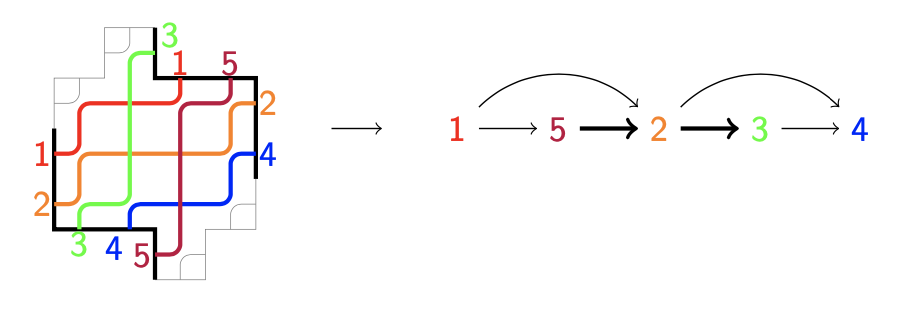
\includegraphics[width=0.52\textwidth]{interval_not_contained1} \quad
	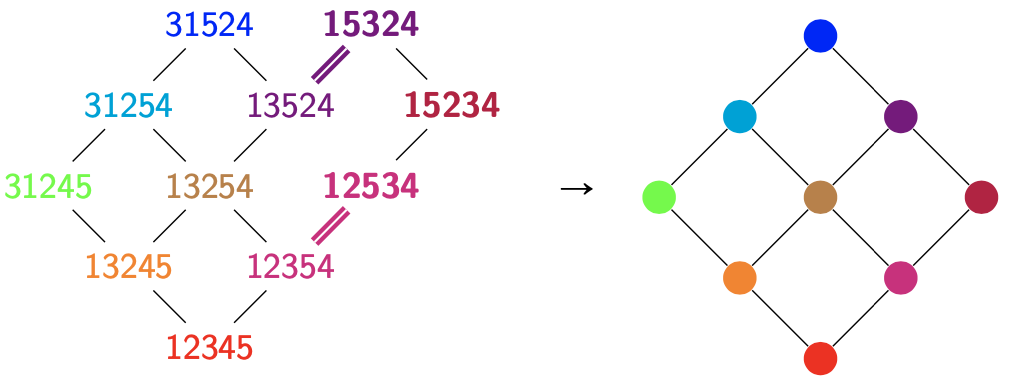
\includegraphics[width=0.43\textwidth]{interval_not_contained2}
	\caption{A facet of a subword complex~$\subwordComplex(Q, \omega)$ whose linear extensions all lie outside the interval~$[e, \omega]$.}
	\label{fig:outOfInterval}
\end{figure}
%
\setcounter{enumi}{3}
\item $\linearExtensions(I)$ is not an interval in general. See for instance the example~\cite[Figure~9]{PilaudStump-brickPolytope}. 
In that figure, the elements of the week order $\mathfrak{S}_4$ that are linear extensions of the same acyclic facet of a given subword complex are grouped together. Some of the groups in the figure are not intervals.  \\
\end{enumerate}
\end{remark}

We will now prove the four points of \cref{thm:linearExtensionsPartitionSubwordComplexA} one by one.

\begin{proof}[Proof of \cref{thm:linearExtensionsPartitionSubwordComplexA}~\eqref{item:convex}]
Let $\sigma < \tau < \rho$ be such that~$\sigma, \rho \in \linearExtensions(I)$.
By definition of linear extensions, we have
\[
\Roots(I) \subseteq \sigma(\Phi^+)=-\Inv(\sigma) \sqcup \Ninv(\sigma)
\quad\text{and}\quad
\Roots(I) \subseteq \rho(\Phi^+)=-\Inv(\rho) \sqcup \Ninv(\rho).
\]
Restricting to the set of negative and positive roots, respectively, we deduce
\[
\Roots(I) \cap \Phi^- \subseteq -\Inv(\sigma) \subseteq -\Inv(\tau) \qquad 
\Roots(I) \cap \Phi^+ \subseteq \Ninv(\rho)  \subseteq \Ninv(\tau)
\]
since~$\sigma < \tau < \rho$. Therefore
\[
\Roots(I) \subseteq -\Inv(\tau) \sqcup \Ninv(\tau) = \tau(\Phi^+)
\]
and so $\tau \in \linearExtensions(I)$.
\end{proof}

\begin{proof}[Proof of \cref{thm:linearExtensionsPartitionSubwordComplexA} \eqref{item:lowerSet}]
Let $\pi \in \linearExtensions(I)$ for some facet $I$.
We need to show that if $\pi' < \pi$ then there exist another facet $I'$ such that $\pi' \in \linearExtensions(I')$.
It is enough to show this when $\pi = \pi's$ for some descent~$s$ of~$\pi$ (\ie some $s\in S$ such that $\ell(\pi') < \ell(\pi)$).

By definition, $\pi \in \linearExtensions(I)$ if and only if $\Roots(I) \subseteq \pi(\Phi^+)$.
Now,
\[
\pi(\Phi^+)= -\Inv(\pi)\sqcup \Ninv(\pi)
\]
and 
\[
\Inv(\pi') =\Inv(\pi) \ssm \{\beta\}
\qquad\text{and}\qquad
\Ninv(\pi') = \Ninv(\pi) \cup \{\beta\}
\]
for $\beta=\pi'(\alpha_s)$.
Therefore,
\begin{align*}
    \pi'(\Phi^+) = \pi(\Phi^+) \ssm \{-\beta\} \cup \{\beta\}.
\end{align*}

\begin{center}
\begin{tikzpicture}
\coordinate (a) at (0,0);
\coordinate (b) at (0:2);
\coordinate (c) at (60:2);
\coordinate (d) at (120:2);
\coordinate (e) at (180:2);
\draw (b) node[right] {$\beta$};
\draw (e) node[left] {$-\beta$};
%
\path[fill=green!20] (0,0) --  (60:2) arc(60:180:2) -- cycle;
%
\draw[-stealth,dashed] (a) -- (b);
\draw[-stealth] (a) -- (c);
% \draw[-stealth] (a) -- (d);
\draw[-stealth] (a) -- (e);
\node at (120:1) {$\pi(\Phi^+)$};
\end{tikzpicture} 
%
\qquad
%
\begin{tikzpicture}
\coordinate (a) at (0,0);
\coordinate (b) at (0:2);
\coordinate (c) at (60:2);
\coordinate (d) at (120:2);
\coordinate (e) at (180:2);
\draw (b) node[right] {$\beta$};
\draw (e) node[left] {$-\beta$};
%
\path[fill=green!20] (0,0) -- (0:2) arc(0:120:2)  -- cycle;
%
\draw[-stealth] (a) -- (b);
% \draw[-stealth] (a) -- (c);
\draw[-stealth] (a) -- (d);
\draw[-stealth,dashed] (a) -- (e);
\node at (60:1) {$\pi'(\Phi^+)$};
\end{tikzpicture} 
\end{center}
%
Note that the reflection $s_\beta=\pi's\pi'^{-1}$ orthogonal to the root $\beta$ transforms $\pi(\Phi^+)$ and $\pi'(\Phi^+)$ into each other:
\[
s_\beta(\pi(\Phi^+))=\pi'(\Phi^+).
\]
Since $s_\beta(\beta)= -\beta$, then $s_\beta$ preserves the set 
\[
\pi(\Phi^+) \ssm \{-\beta\} = \pi'(\Phi^+) \ssm \{\beta\} = \pi(\Phi^+) \cap \pi'(\Phi^+).
\]
This observation will be useful to prove the statement in the second of the following two cases.
\vincent{I believe we could shorten all this discussion. Also the picture is not really useful.}

\medskip
\paragraph{\bf Case 1:} $-\beta \notin \Roots(I)$.

In this case, 
$\Roots(I)\subseteq \pi(\Phi^+) \ssm \{-\beta\} \subseteq \pi'(\Phi^+)$.
Taking $I'=I$, we have 
$\pi'\in \linearExtensions(I')$ 
as wanted.

\medskip
\paragraph{\bf Case 2:} $-\beta \in \Roots(I)$.

In this case, we need to remove $-\beta$ from the root configuration.
We will achieve this by flipping the position of the last $-\beta$ in $I$ to create a new facet $I'$.
This position is indeed flippable as we will argue now. 

Given a facet $I$ of a subword complex~$\subwordComplex(Q,\omega)$ and a positive root $\beta\in \Phi^+$, the restriction of the list of roots 
\[
\rootFunction{I}{1}, \rootFunction{I}{2}, \dots , \rootFunction{I}{m}.
\]
to the set $\{\beta,-\beta\}$ is of the form
\[
\begin{array}{cccc}
  \beta, \dots , & \beta &, -\beta, \dots, &-\beta.\\
     & i && j
\end{array}
\]
The sequence of $-\beta$'s could in principle be empty and so does the sequence of $\beta$'s.
But if there is a $-\beta$ in this list, then there should be at least one $\beta$ preceding it.
The position $i$ of the last $\beta$ is used in the reduced expression of $\omega$ in the complement of $I$, that is $i\notin I$.
The positions of the other $\beta$'s and $-\beta$'s all belong to~$I$, and can all be flipped to $i$ (see \cref{lem:rootFunctionFlips}~\eqref{lem:rootFunctionFlips2}).   
In particular, the position $j$ of the last $-\beta$ belongs to $I$, and it can be flipped to $i$ creating a new facet $I'=I\ssm \{j\} \cap \{i\}$.

Now, since $\beta\notin \pi(\Phi^+)$.
There must be only one $\beta$ in the list.
Otherwise, there would be at least one $\beta$ whose position belongs to the facet $I$.
This would imply that $\beta\in \Roots(I)$ and $\pi$ would not be a linear extension of $I$, which is a contradiction.
So, our restricted list corresponding to $I$ looks like
\begin{equation}
\begin{array}{ccc}
  \beta &, -\beta, \dots, &-\beta.\\
      i && j
\end{array}    
\end{equation}
By  \cref{lem:rootFunctionFlips}~\eqref{lem:rootFunctionFlips3}, we obtain that flipping $j$ to $i$ creates the new facet $I' = I \ssm \{j\} \cap \{i\}$ whose corresponding restricted list looks like
\begin{equation}
\begin{array}{ccc}
  \beta &, \beta, \dots, &\beta.\\
      i && j
\end{array}    
\end{equation}

Moreover, since the reflection $s_\beta$ preserves the set 
\[
\pi'(\Phi^+) \ssm \{\beta\} = \pi(\Phi^+) \ssm \{-\beta\} = \pi(\Phi^+) \cap \pi'(\Phi^+).
\]
then $\Roots(I') \subseteq \pi'(\Phi^+)$.
Thus, $\pi'\in \linearExtensions(I')$ as desired.
\end{proof}

\begin{proof}[Proof of \cref{thm:linearExtensionsPartitionSubwordComplexA}~\eqref{item:cover}]
By part \eqref{item:lowerSet}, the union of all linear extensions of facets is a lower set.
So, we just need to show that $\omega$ belongs to this set.
This follows from $\omega\in \linearExtensions(\antiGreedyFacet)$, which was proven in \cref{lem:linearExtensionsGreedyFacets}.
\end{proof}

\begin{proof}[Proof of \cref{thm:linearExtensionsPartitionSubwordComplexA}~\eqref{item:partition}]
We show that if there is two facets~$I_1, I_2$ of~$\subwordComplex(Q, \omega)$ and an element~$\pi \in W$ such that $\pi \in \linearExtensions(I_1) \cap \linearExtensions(I_2)$ then~$I_1= I_2$.
The proof works by induction on the length~$\ell(\pi)$ of~$\pi$.
We already showed this for $\pi = e$ in \cref{lem:linearExtensionsGreedyFacets}.

Let $I_1, I_2$ be two facets such that $e \neq \pi \in \linearExtensions(I_1)\cap \linearExtensions(I_2)$.
As in the proof of part \eqref{item:lowerSet}, let $\pi'=\pi s$ for some $s\in S$ such that $\ell(\pi')<\ell(\pi)$, and let $I_1',I_2'$ be the corresponding facets obtained using the same steps of the proof.
These new facets satisfy $\pi' \in \linearExtensions(I_1')\cap \linearExtensions(I_2')$, so that~$I_1' = I_2'$ by induction.

We now claim that it implies that~$I_1 = I_2$.
We analyze the two cases if the proof of part \eqref{item:lowerSet}.
Note that in Case~1, the resulting facet~$I'$ obtained from $I$ satisfies $\beta\notin \Roots(I')$, while in Case 2 we have $\beta \in \Roots(I')$. 
As $I_1' = I_2'$, this shows that $I_1$ and $I_2$ fall either both into Case 1 or both into Case 2.
If both fall into Case 1, then $I_1'=I_1$ and $I_2'=I_2$ and so $I_1=I_2$ as desired.
If both fall into Case 2, then we just need to flip back the performed flip to obtain $I_1=I_2$.
\end{proof}

Since $\linearExtensions(I)\neq \varnothing$ if and only if $I$ is acyclic by \cref{lem:linearExtensionsAcyclic}, and~$\linearExtensions(I) \ne \linearExtensions(J)$ for~$I \ne J$ by \cref{thm:linearExtensionsPartitionSubwordComplexA}~\eqref{item:partition}, we have the following straight forward corollary.

\begin{corollary}
\label{coro:linearExtensionsPartitionSubwordComplexes}
For any word~$Q$ and element~$\omega$,
\[
\linearExtensions(Q,\omega) = \bigsqcup_{I\in\subwordAcyclicFacets(Q,\omega)} \linearExtensions(I).
\]
\end{corollary}

As pointed out in \cref{rem:linearExtensionsPartitionSubwordComplexA}, there are subword complexes for which $[e,\omega] \neq \linearExtensions(Q,\omega)$.
Our second fundamental theorem describes a large family of cases where equality holds.
We say that a word~$Q$ is \defn{sorting} if it contains a reduced expression of $\wo$.
Equivalently~$Q$ contains a reduced expression for any element~$w \in W$.
Still equivalently, $\DemazureProduct(Q) = \wo$ where~$\DemazureProduct(Q)$ denotes the \defn{Demazure product} of~$Q$, defined by~$\DemazureProduct(\varepsilon) = e$ and~$\DemazureProduct(Qs) = \max(\DemazureProduct(Q), \DemazureProduct(Q)s)$ (where the $\max$ is in weak order).

\begin{theorem}
\label{thm:linearExtensionsPartitionSubwordComplexB}
If the word $Q$ is sorting, then the linear extensions of acyclic facets of $\subwordComplex(Q,\omega)$ form a partition of the interval $[e,\omega]$, that is
\[
[e,\omega] = \bigsqcup_{I\in\subwordAcyclicFacets(Q,\omega)} \linearExtensions(I).
\]
\end{theorem}

The proof is based on the following statement, which follows from~\cite[Thm.~3.1 \& Coro.~3.3]{JahnStump}.

\begin{proposition}[{\cite{JahnStump}}]
\label{prop:intersectionRootConfigurations}
If the word $Q$ is sorting, then 
\[
\Big( \bigcap_{I\in \subwordFacets(Q,\omega)} \cone \Roots(I) \Big) \cap \Phi^+ = \Ninv(\omega).
\]
\end{proposition}

\begin{proof}
We include a short proof here for self containment.
We refer to~\cite{JahnStump} for the description of the notation $C^+(\omega,\cdot)$.
By~\cite[Theorem~3.1]{JahnStump} we have
\[
\bigcap_{I\in \subwordFacets(Q,\pi)} \cone \Roots(I) = C^+(\omega,\DemazureProduct(Q)).
\]
The word $Q$ contains a reduced expression of $\wo$ if and only if $\DemazureProduct(Q)=\wo$.
Furthermore, by~\cite[Corollary~3.3]{JahnStump} we have
\[
C^+(\omega,\wo)\cap \Phi^+ = \Inv(\omega \wo) = \Ninv(\omega).
\qedhere
\]
\end{proof}

\begin{proof}[Proof of \cref{thm:linearExtensionsPartitionSubwordComplexB}]
If $\pi \in \linearExtensions(I)$ for some facet~$I$ of~$\subwordComplex(Q, \omega)$, then by \cref{prop:intersectionRootConfigurations} we have 
\[
\Ninv(\omega) \subseteq \cone \Roots(I) \cap \Phi^+ \subseteq \cone \pi(\Phi^+) \cap \Phi^+  = \Ninv(\pi).
\]
Thus $\pi \le \omega$ as desired.
\end{proof}

%%%%%%%%%%%%%%%%%%%%%%%%%%%%%%%%%%%%%%

\subsection{Five conjectures on linear extensions of facets}
\label{subsec:fiveConjectures}

In this section, we present conjectural generalizations of the results of \cref{subsec:pipeDreamCongruence,subsec:pipeDreamQuotient}.
By \cref{coro:linearExtensionsPartitionSubwordComplexes}, we have
\[
\linearExtensions(Q,\omega) = \bigsqcup_{I \in \subwordAcyclicFacets(Q, \omega)} \linearExtensions(I)
\]
which naturally defines an equivalence relation on~$\linearExtensions(Q,\omega)$.
However, this equivalence relation is in general not a lattice congruence for two obvious reasons:
\begin{enumerate}[(i)]
\item while~$\linearExtensions(Q,\omega)$ is a lower set of the weak order containing~$[e, \omega]$ by \cref{thm:linearExtensionsPartitionSubwordComplexA}, it does not always coincides with~$[e, \omega]$ by \cref{rem:linearExtensionsPartitionSubwordComplexA}, and in fact it does not necessarily have a maximal element, hence it is not necessarily a lattice,
\item while the sets~$\linearExtensions(I)$ are always order convex in the weak order by \cref{thm:linearExtensionsPartitionSubwordComplexA}~\eqref{item:convex}, they are not necessarily intervals in the weak order by \cref{rem:linearExtensionsPartitionSubwordComplexA}.
\end{enumerate}
To bypass Issue~(i), we could restrict our attention to the situation when the word~$Q$ is sorting by~\cref{thm:linearExtensionsPartitionSubwordComplexB} (we will do that in \cref{conj:latticeQuotientSortingAlternating}).
Here, we want to be slightly more general, so we will instead consider general words~$Q$, but restrict our attention to the interval~$[e, \omega]$ as follows.
For a facet~$I$ of~$\subwordComplex(Q, \omega)$, we define~$\strongLinearExtensions(I) \eqdef \linearExtensions(I) \cap [e, \omega]$.
We say that~$I$ is \defn{strongly acyclic}~$\strongLinearExtensions(I) \ne \varnothing$, and we denote by~$\subwordStronglyAcyclicFacets(Q, \omega)$ the set of strongly acyclic facets of~$\subwordComplex(Q, \omega)$.
Note that by \cref{thm:linearExtensionsPartitionSubwordComplexA}~\eqref{item:partition}, we have
\[
[e, \omega] = \bigsqcup_{I\in\subwordStronglyAcyclicFacets(Q,\omega)} \strongLinearExtensions(I).
\]
We can thus now define the analogue of the pipe dream congruence of \cref{def:pipeDreamCongruence} for subword complexes as follows.

\begin{definition}
\label{def:pipeDreamCongruenceSubwordComplexes}
For a non-empty subword complex $\subwordComplex(Q,\omega)$, the \defn{subword complex congruence} is the equivalence relation~$\equiv_{Q,\omega}$ on the interval~$[e, \omega]$  whose equivalence classes are the sets~$\strongLinearExtensions(I)$ of linear extensions of strongly acyclic facets~$I$ of~$\subwordStronglyAcyclicFacets(Q, \omega)$.
In other words, $\pi \equiv_{Q,\omega} \pi'$ if and only if $\pi$ and $\pi'$ are linear extensions of the same facet.  
\end{definition}

Despite its name, this equivalence relation is not always a congruence because of Issue~(ii) above.
To fix it, we now assume that the word~$Q$ is \defn{alternating}, meaning that all non-commuting pairs $s, t\in S$ alternate within $Q$ (this notion was already considered in \cite{PilaudSantos-brickPolytope, CeballosLabbeStump}).
This enables us to state our first conjecture, intended to extend~\cref{thm:pipeDreamCongruence}.

\begin{conjecture}
\label{conj:latticeCongruenceAlternating}
For a non-empty subword complex $\subwordComplex(Q,\omega)$ where~$Q$ is alternating, the subword complex congruence~$\equiv_{Q,\omega}$ is a lattice congruence of the interval~$[e,\omega]$ of the weak order.
\end{conjecture}

We now intend to understand the quotient~$[e, \omega]/\equiv_{Q, \omega}$.
First, its elements correspond to the congruence classes of~$\equiv_{Q, \omega}$, hence to the strongly acyclic facets in~$\subwordStronglyAcyclicFacets(Q, \omega)$.
The cover relations are certain increasing flips between the facets in~$\subwordStronglyAcyclicFacets(Q, \omega)$.
However, in contrast to \cref{thm:pipeDreamQuotient}, not all increasing flips between two facets in~$\subwordStronglyAcyclicFacets(Q, \omega)$ yields a cover relation of~$\subwordStronglyAcyclicFacets(Q, \omega)$, as illustrated by the following example.

\begin{example}
\label{exm:acyclicFlipvsWeakOrder}
Consider the type~$A_2$ Coxeter system, the word~$Q = \tau_1 \tau_2 \tau_1 \tau_2 \tau_1 \tau_2$ and the longest element~$\wo = \tau_1 \tau_2 \tau_1 = \tau_2 \tau_1 \tau_2$.
The subword complex~$\subwordComplex(Q, \wo)$ has eight facets, six of which are acyclic.
All the fibers of $\equiv_{Q, \wo}$ are singletons and the lattice quotient~$[e, \wo]/\equiv_{Q, \wo}$ coincides with the weak order of type~$A_2$.
Note that the two acyclic facets~$\{1,3,4\}$ and $\{3,4,6\}$ are connected by a flip but the corresponding classes do not form a cover relation in~$[e, \wo]/\equiv_{Q, \wo}$.
%
\begin{figure}[h]
	\begin{tikzpicture}[xscale=1.5,->]
	\node (123) at (0,-2.5) {$\{1,2,3\}$};
	\node (134) at (-1,-1.5) {$\{1,3,4\}$};
	\node (126) at (0.3,-.5) {$\{1,2,6\}$};
	\node (236) at (1,-1.5) {$\{2,3,6\}$};
	\node (145) at (-1,1.5) {$\{1,4,5\}$};
	\node (156) at (-0.3,.5) {$\{1,5,6\}$};
	\node (346) at (1,1.5) {$\{3,4,6\}$};
	\node (456) at (0,2.5) {$\{4,5,6\}$};
	\draw (123)--(134);
	\draw (123)--(126);
	\draw (123)--(236);
	\draw (134)--(145);
	\draw (134)--(346);
	\draw (126)--(156);
	\draw (236)--(126);
	\draw (236)--(346);
	\draw (145)--(456);
	\draw (156)--(145);
	\draw (156)--(456);
	\draw (346)--(456);
	\end{tikzpicture}
	\qquad
	\begin{tikzpicture}[xscale=1.5,->]
	\node (123) at (0,-2.5) {$\{1,2,3\}$};
	\node (134) at (-1,-1.5) {$\{1,3,4\}$};
	\node (236) at (1,-1.5) {$\{2,3,6\}$};
	\node (145) at (-1,1.5) {$\{1,4,5\}$};
	\node (346) at (1,1.5) {$\{3,4,6\}$};
	\node (456) at (0,2.5) {$\{4,5,6\}$};
	\draw (123)--(134);
	\draw (123)--(236);
	\draw (134)--(145);
	\draw (134)--(346);
	\draw (236)--(346);
	\draw (145)--(456);
	\draw (346)--(456);
	\end{tikzpicture}
	\qquad
	\begin{tikzpicture}[xscale=1.5,->]
	\node (123) at (0,-2.5) {$\{1,2,3\}$};
	\node (134) at (-1,-1.5) {$\{1,3,4\}$};
	\node (236) at (1,-1.5) {$\{2,3,6\}$};
	\node (145) at (-1,1.5) {$\{1,4,5\}$};
	\node (346) at (1,1.5) {$\{3,4,6\}$};
	\node (456) at (0,2.5) {$\{4,5,6\}$};
	\draw (123)--(134);
	\draw (123)--(236);
	\draw (134)--(145);
	\draw (236)--(346);
	\draw (145)--(456);
	\draw (346)--(456);
	\end{tikzpicture}
	\caption{The increasing flip graph on~$\subwordComplex(Q, \wo)$ (left), its restriction to acyclic facets (middle) and the Hasse diagram of the quotient~$[e, \wo]/\equiv_{Q, \wo}$ where each class is labeled by its corresponding facet of~$\subwordComplex(Q, \wo)$ (right), for the subword complex~$\subwordComplex(Q, \wo)$ where~$Q = \tau_1 \tau_2 \tau_1 \tau_2 \tau_1 \tau_2$ and~$\wo = \tau_1 \tau_2 \tau_1 = \tau_2 \tau_1 \tau_2$. Note that the increasing flip~$\{1,3,4\} \to \{3,4,6\}$ is not a cover relation of~$[e, \wo]/\equiv_{Q, \wo}$.}
	\label{fig:acyclicFlipvsWeakOrder}
\end{figure}
\end{example}

We say that a flip between two facets~$I, J \in \subwordStronglyAcyclicFacets(Q, \omega)$ with~$I \ssm \{i\} = J \ssm \{j\}$ is \defn{extremal} if the root~$\rootFunction{I}{i}$ is a ray of the root configuration~$\Roots(I)$ (or equivalently, $\rootFunction{J}{j}$ is a ray~$\Roots(J)$).
This enables us to state our second conjecture, intended to extend~\cref{thm:pipeDreamQuotient}.

\begin{conjecture}
\label{conj:latticeQuotientAlternating}
For a non-empty subword complex $\subwordComplex(Q,\omega)$ where~$Q$ is alternating, the Hasse diagram of the lattice quotient~$[e, \omega]/\equiv_{Q, \omega}$ is isomorphic to the graph of extremal increasing flips between strongly acyclic facets of~$\subwordStronglyAcyclicFacets(Q, \omega)$.
\end{conjecture}

We now specialize \cref{conj:latticeCongruenceAlternating,conj:latticeQuotientAlternating} to the case of sorting and alternating words.
In this case, all acyclic facets are strongly acyclic by \cref{thm:linearExtensionsPartitionSubwordComplexB}.
Note that this is precisely the situation we had in~\cref{sec:latticeAcyclicPipeDreams}.

\begin{conjecture}
\label{conj:latticeQuotientSortingAlternating}
If~$Q$ is sorting and alternating, then the Hasse diagram of the lattice quotient~$[e, \omega]/\equiv_{Q, \omega}$ is isomorphic to the graph of extremal increasing flips between acyclic facets of~$\subwordAcyclicFacets(Q, \omega)$.
\end{conjecture}

Moreover, there is a close connection with the brick polyhedra introduced in~\cite{JahnStump} as generalizations of the brick polytopes of~\cite{PilaudSantos-brickPolytope, PilaudStump-brickPolytope}.
We refer to the original papers~\cite{PilaudSantos-brickPolytope, PilaudStump-brickPolytope, JahnStump} for a definition of these polyhedra.
We just need to know here that the brick polyhedron~$\brickPolyhedron(Q, \omega)$~has
\begin{itemize}
\item a vertex for each acyclic facet of~$\subwordAcyclicFacets(Q, \omega)$, and
\item an edge for each extremal flip between two acyclic facets,
\end{itemize}
and that the graph of extremal increasing flips on acyclic facets is isomorphic to the finite part (meaning forgetting the unbounded rays) of the graph of the brick polyhedron~$\brickPolyhedron(Q, \omega)$ oriented in a suitable direction~$\delta$.
This can be derived from \cite[Thm.~4.4]{JahnStump}.
\cref{conj:latticeQuotientSortingAlternating} can thus be translated geometrically as follows.

\begin{conjecture}
\label{conj:latticeQuotientSortingAlternatingBrickPolyhedra}
If~$Q$ is sorting and alternating, then the finite part of the oriented graph of the brick polyhedron~$\brickPolyhedron(Q, \omega)$ is isomorphic to the Hasse diagram of the lattice quotient~$[e, \omega]/\equiv_{Q, \omega}$.
\end{conjecture}

In particular, specializing this conjecture to the brick polytopes~\cite{PilaudSantos-brickPolytope, PilaudStump-brickPolytope} for which~$\omega = \wo$, we obtain our last conjecture, intended to extend the results of~\cite{Pilaud-brickAlgebra}.

\begin{conjecture}
\label{conj:latticeQuotientSortingAlternatingBrickPolytopes}
If~$Q$ is sorting and alternating, then the oriented graph of the brick polytope~$\brickPolyhedron(Q, \wo)$ is isomorphic to the Hasse diagram of a lattice quotient of the weak order.
\end{conjecture}

\begin{remark}
\cref{conj:latticeCongruenceAlternating,conj:latticeQuotientAlternating,conj:latticeQuotientSortingAlternating,conj:latticeQuotientSortingAlternatingBrickPolyhedra,conj:latticeQuotientSortingAlternatingBrickPolytopes} holds in type~$A_n$: our specific proof of~\cref{thm:pipeDreamCongruence,thm:pipeDreamQuotient} can be extended to arbitrary alternating words in type~$A_n$ as will be shown in~\cite{Cartier}.
They are also supported by computer experiments: we verified \cref{conj:latticeCongruenceAlternating,conj:latticeQuotientAlternating} for all alternating words of length at most~$\ell(\wo)$ (hence \cref{conj:latticeQuotientSortingAlternating,conj:latticeQuotientSortingAlternatingBrickPolyhedra,conj:latticeQuotientSortingAlternatingBrickPolytopes} for all alternating reduced expressions of~$\wo$) in types~$B_2, B_3, D_4$ and~$H_3$.
\end{remark}



\vincent{I want to delete the remaining of this section, but I want to discuss it with Cesar.}

As we have seen in \cref{cor_acyclicpipedreams_lattice}, the increasing flip poset of acyclic pipe dreams of any permutation $\omega$ is a lattice, because it is isomorphic to the lattice quotient~$[e,\omega]/\equiv_\omega$.
This motivates the following open question for subword complexes.

\begin{question}
Let $\subwordComplex(Q,\omega)$ be a non-empty subword complex.
Is the restriction of the increasing flip poset of $\subwordComplex(Q,\omega)$ to the set of acyclic facets a lattice?    
\end{question}

As pointed out in \cref{rem_acyclicflipposet_not_latticequotient},  we can not expect~$[e,\omega]/\equiv_{Q,\omega}$ to be isomorphic to the restriction of the increasing flip poset of $\subwordComplex(Q,\omega)$ to the set of acyclic facets.
\cref{exm:acyclicFlipvsWeakOrder} shows that there are flips between acyclic facets that are not detected by the week order.
One could expect that there is a natural restriction to a special class of flips that behave nicer, meaning that all of them are identified by the quotient~$[e,\omega]/\equiv_{Q,\omega}$.
In our \cref{exm:acyclicFlipvsWeakOrder}, the generalized Chute moves from~\cite{Rubey} do the job, because the flip that is not detected by the week order is exactly the one flip which is not Chute.
The Chute lattice conjecture~\cite[Conjecture~2.8]{Rubey} might be an indication that this is the right direction to look at.

%%%%%%%%%%%%%%%%%%%%%%%%%%%%%%%%%%%%%%

\subsection{The sweeping algorithm}
\label{subsec:sweepingAlgorithmSubwordComplexes}
\vincent{I have not checked this part yet.}
\vincent{Here, we must properly cite \cite{JahnStump} and say that we obtained this algorithm independently.}

Given a linear extension $\pi \in \linearExtensions(Q,\omega)$, one natural question is whether we can recover the unique acyclic facet $I$ such that $\pi \in \linearExtensions(I)$.
We can recover this facet via a sweeping algorithm which we now introduce.
The algorithm outcomes a facet for every element~$\pi \in W$, and this will be the desired facet for each $\pi \in \linearExtensions(Q,\omega)$.

\[
\begin{tabular}{cccc}
$\sweepingAlgorithm$ : & $W$  &$\longrightarrow$ &$\subwordFacets(Q,\omega)$\\
    & $\pi$ & $\longrightarrow$ & $\sweepingAlgorithm(Q,\omega,\pi)$
\end{tabular}
\]

We start by setting $I^0=\varnothing$ to be the empty set.
Then we scan the word $Q=(q_1,\dots ,q_m)$ from left to right.
At position $j\in [m]$ we produce a new set $I^j$ obtained from the previous one $I^{j-1}$ by either adding $j$ or not, according to certain rules.
We let $Q^j=Q_{[j]\ssm I^j}$ and denote by
    \[
    \rootFunction{I^j}{k} = \prod Q_{[k-1]\ssm I^j}(\alpha_{q_k}).
    \]
the partial root function for $k\leq j$.  
The rules are the following:

\begin{enumerate}
    \item If $\rootFunction{I^j}{j}\in \Ninv(\omega)$ then let 
    \[
    I^j=I^{j-1}\cup\{j\}.
    \] 
    \label{sweeping_case1}
    \item If $\rootFunction{I^j}{j}\in \Inv(\omega) \cap \Inv (\pi)$ then let 
    \[
    I^j=I^{j-1}.
    \]
    \label{sweeping_case2}
    \item If $\rootFunction{I^j}{j}\in \Inv(\omega) \cap \Ninv (\pi)$ then we consider two cases: 
    \label{sweeping_case3} 
    \begin{enumerate}
        \item If $Q_{[m]\ssm I^{j-1}\ssm \{j\}}$ contains a reduced expression of $\omega$ with prefix $Q^{j-1}$ then let 
        \[
        I^j=I^{j-1}\cup \{j\}.
        \]        
        \label{sweeping_case3a}
        \item If not let 
        \[
        I^j=I^{j-1}.
        \]
        \label{sweeping_case3b}
    \end{enumerate}
    \item If $\rootFunction{I^j}{j}\in -\Inv(\omega)$ then let
    \[
    I^j=I^{j-1}\cup \{j\}.
    \]
    \label{sweeping_case4}
\end{enumerate}

We denote by \defn{$\sweepingAlgorithm(Q,\omega,\pi)$} the resulting set $I^m$ obtained at the last step of the algorithm.

Roughly speaking, the goal of the algorithm is to insert a reduced expression of $\omega$ in $Q$ by sweeping the word from left to right, while deciding whether we use a letter or not by looking at the root $\beta=\rootFunction{I^j}{j}$ that it produces.
If $\beta \in \Ninv(\omega)$ then it can not be used (Case~\eqref{sweeping_case1}), otherwise we would not have a reduced expression for $\omega$.
If $\beta \in \Inv(\omega)$ then we take it when $\beta \in \Inv(\pi)$ (Case~\eqref{sweeping_case2}), or delay it as much as possible when $\beta \in \Ninv(\pi)$ (Case~\eqref{sweeping_case3}).
If $\beta \in -\Inv(\omega)$ we can simply not take it (Case~\eqref{sweeping_case4}).

\begin{proposition}
\label{prop_sweeping1}
    Let $\subwordComplex(Q,\omega)$ be a non-empty subword complex.
    For every $\pi \in W$, the set $\sweepingAlgorithm(Q,\omega,\pi)$ is a facet of $\subwordComplex(Q,\omega)$.
\end{proposition}

\begin{proof}
    Let $I^j$ and $Q^j=Q_{[j]\ssm I^j}$ be as defined in the sweeping algorithm for $\pi$. 
    The proposition follows by applying the following claim for $j=m$.
    \smallskip
    
    {\bf Claim}: $Q^j$ is a reduced expression which is the prefix of a reduced expression of $\omega$ in $Q_{[m]\ssm I^j}$.

    \smallskip
    We prove the claim by induction on $j$.

    For $j=0$, $Q^0$ is the empty word which is reduced by definition.
    Furthermore, $Q_{[m]\ssm I^0 }=Q$ contains a reduced expression of $\omega$ because the subword complex is non-empty.
The empty word is a prefix of this reduced expression. 

    Now assume that the claim holds for $j-1$ and prove it for $j$.
    Note that 
    \begin{equation}
         Q^j = 
  \begin{cases}
    Q^{j-1}, & \text{if } I^j=I^{j-1}\cup \{j\} \\
    Q^{j-1}\circ (q_j), & \text{if } I^j=I^{j-1}
  \end{cases}
    \end{equation}    
    We analyze the different cases of the sweeping algorithm.
    \begin{enumerate}
    \item If $\rootFunction{I^j}{j}\in \Ninv(\omega)$ then 
    $Q^j=Q^{j-1}$, which is reduced by induction hypothesis.
    Moreover, it is a prefix of a reduced expression of $\omega$ in $Q_{[m]\ssm I^{j-1}}$.
    Since $\rootFunction{I^j}{j}\in \Ninv(\omega)$, this reduced expression can not use the letter $q_j$; so, it is a reduced expression of $\omega$ in $Q_{[m]\ssm I^{j}}$ as desired.
    \item If $\rootFunction{I^j}{j}\in \Inv(\omega) \cap \Inv (\pi)$ then $Q^j= Q^{j-1}\circ (q_j)$, which is a reduced expression because~$Q^{j-1}$ is reduced and $\rootFunction{I^j}{j}\in \Inv(\omega)$.
    
    Now let $\widetilde Q$ be a subword of $Q_{[m]\ssm I^{j-1}}=Q_{[m]\ssm I^{j}}$ which is a reduced expression of $\omega$ with prefix $Q^{j-1}$, and let $\widetilde I$ be the corresponding facet.
    
    If $j\notin \widetilde I$, then $q_j$ is used in $\widetilde Q$ and we are done because $\widetilde Q$ has $Q^j$ as a prefix.

    If $j\in \widetilde I$, then we can flip it to a position $j'>j$ (by \cref{lem:rootFunctionFlips}~\eqref{lem:rootFunctionFlips2}), creating a new reduced expression $\widetilde Q'$ of $\omega$ which uses $q_j$, and thus has $Q^j$ as a prefix.


    \item[(3)(a)] If $\rootFunction{I^j}{j}\in \Inv(\omega) \cap \Ninv (\pi)$ and $Q_{[m]\ssm I^{j-1}\ssm \{j\}}$ contains a reduced expression of $\omega$ with prefix $Q^{j-1}$, then $Q^j=Q^{j-1}$.
    Therefore, $Q^j$ is reduced and it is a prefix of a reduced expression of $\omega$ in 
    $Q_{[m]\ssm I^{j-1}\ssm \{j\}}=Q_{[m]\ssm I^j}$.

    \item[(3)(b)] In this case, $\rootFunction{I^j}{j}\in \Inv(\omega) \cap \Ninv (\pi)$ but $Q^j= Q^{j-1}\circ (q_j)$. The proof is similar to the proof of (2).

    \item[(4)] If $\rootFunction{I^j}{j}\in -\Inv(\omega)$ then $Q^j=Q^{j-1}$. The argument is similar to that of part (1).
    \end{enumerate}

Finally, we need to argue that any position $j$ falls into one of these cases.
The root $\rootFunction{I^j}{j}\in \Phi^+ \sqcup \Phi^-$ and we know that
\[
\Phi^+ = \Inv(\omega) \sqcup \Ninv(\omega) \qquad \qquad
\Phi^- = -\Inv(\omega) \sqcup -\Ninv(\omega)  
\]
The positive roots are covered by the cases (1),(2), and (3).
The negative roots in $-\Inv(\omega)$ are covered in case (4).
Since we are inserting a reduced expression of $\omega$ in $Q$, the case $-\Ninv(\omega)$ never occurs. 
\end{proof}

The following proposition shows that for every linear extension $\pi \in \linearExtensions(Q,\omega)$, the sweeping algorithm recovers the unique acyclic facet $I$ such that $\pi \in \linearExtensions(I)$.

\begin{proposition}
\label{prop_sweeping2}
    If $\pi\in \linearExtensions(I)$ for some facet $I\in \subwordComplex(Q,\omega)$, then 
    \[
I = \sweepingAlgorithm(Q,\omega,\pi).
    \]
\end{proposition}

Our proof is based on the following lemma.

\begin{lemma}\label{lem_negativeroot}
    Let $I_1,I_2\in \subwordComplex(Q,\omega)$ be two different facets, and $j\in [m]$ be the first position where they differ.
    Without loss of generality assume 
    \[
I_2\cap [j] = I_1\cap [j] \ssm \{j\}
    \]
with $j\in I_1$.
Let $\beta=\rootFunction{I_1}{j}=\rootFunction{I_2}{j}$, then 
\[
-\beta \in \cone \Roots(I_2).
\]
\end{lemma}

\begin{proof}
    ~\cesar{Noemie: can you please write the proof of this Lemma? I do not remember the details at the moment, but the proof is based on the paper of Jahn--Stump that we discussed during your visit in Graz.}
\end{proof}

\begin{proof}[Proof of \cref{prop_sweeping2}]
Assume $\pi \in \linearExtensions(I)$ and let $I^j=I\cap [j]$.
We will show that the partial root function $\rootFunction{I^j}{\cdot}$ agrees with the decisions taken in the sweeping algorithm.
Indeed, we will see that those decisions are forced.

Recall that 

\begin{center}
\begin{tabular}{ccl}
    $\pi \in \linearExtensions(I)$ & $\longleftrightarrow$ & $R(I)\subseteq \pi(\Phi^+)$\\
     & $\longleftrightarrow$ & $\cone R(I)\subseteq \pi(\Phi^+)$
\end{tabular}    
\end{center}
and 
\[
\pi(\Phi^+) = -\Inv(\pi) \sqcup \Ninv(\pi).
\]
We analyze the possible cases in the sweeping algorithm.

\begin{enumerate}
    \item If $\rootFunction{I^j}{j}\in \Ninv(\omega)$ then clearly $j\in I$ is forced. Otherwise $Q_{[m]\ssm I}$ would not be a reduced expression of $\omega$.
    \item If $\rootFunction{I^j}{j}\in \Inv(\omega) \cap \Inv (\pi)$ then $j\notin I$ is forced. 
    Otherwise we would have an inversion of $\pi$ in the root configuration, which contradicts $\pi \in \linearExtensions(I)$.
    \item[(3)(a)] If $\rootFunction{I^j}{j}\in \Inv(\omega) \cap \Ninv (\pi)$ and $Q_{[m]\ssm I^{j-1}\ssm \{j\}}$ contains a reduced expression of $\omega$ with prefix $Q^{j-1}$ then $j\in I^j$ is forced. 

    We argue this by contradiction. 
    Assume $j\notin I^j$ ($j\notin I$). Let $I_1=\sweepingAlgorithm(Q,\omega,\pi)$ and $I_2=I$. Applying \cref{lem_negativeroot}, we deduce that $\beta=\rootFunction{I^j}{j}=\rootFunction{I}{j}$ satisfies 
    \[
    -\beta \in \cone \Roots(I).
    \]
    But $\beta \in \Ninv(\pi)$. This contradicts $\pi\in \linearExtensions(I)$.
    \item[(3)(b)]  If $\rootFunction{I^j}{j}\in \Inv(\omega) \cap \Ninv (\pi)$ and $Q_{[m]\ssm I^{j-1}\ssm \{j\}}$ does not contain a reduced expression of $\omega$ with prefix $Q^{j-1}$ then $j\notin I^j$ is forced. Otherwise, the complement of $I$ would not be a reduced expression of $\omega$.
    \item[(4)] If $\rootFunction{I^j}{j}\in -\Inv(\omega)$ then $j\in I^j$ is clearly forced. Otherwise, the complement of $I$ would not be a reduced expression.
\end{enumerate}
\end{proof}

\begin{remark}
    Although the sweeping algorithm produces a facet $I=\sweepingAlgorithm(Q,\omega,\pi)$ for every~$\omega\in W$, in some cases we have $\pi \notin \linearExtensions(I)$. 
    This happens because of Case~\eqref{sweeping_case1}, when a non-inversion~$\beta\in \Ninv(\omega)$ of $\omega$ is added to the root configuration $\Roots(I)$, such that~$\beta \notin \Ninv(\pi)$. This is only potentially possible when $\pi \notin [e,\omega]$.
\end{remark}

%%%%%%%%%%%%%%%%%%%%%%%%%%%%%%%%%%%%%%
%%%%%%%%%%%%%%%%%%%%%%%%%%%%%%%%%%%%%%
%%%%%%%%%%%%%%%%%%%%%%%%%%%%%%%%%%%%%%

\bibliographystyle{alpha}
\bibliography{latticePipeDreams}
\label{sec:biblio}

%%%%%%%%%%%%%%%%%%%%%%%%%%%%%%%%%%%%%%

\end{document}
